%ME800401
%Module 1:
%Graphs and level sets, vector fields, the tangent space, surfaces, vector fields on surfaces, orientation.
%(Chapters 1 to 5 of \cite{thorpe}) (20 hours)
%Module 2:
%The Gauss map, geodesics, Parallel transport,
%(Chapters 6, 7 & 8 of \cite{thorpe}) (20 hours)
%Module 3:
%The Weingarten map, curvature of plane curves, Arc length and line integrals
%(Chapters 9, 10 & 11 of \cite{thorpe}) (25 hours)
%Module 4:
%Curvature of surfaces and Parametrized surfaces
%(Chapters 12 & 14 of \cite{thorpe}) (25 hours)

%Module 1 - \cite{thorpe} 1, 2, 3, 4, 5
%Module 2 - \cite{thorpe} 6, 7, 8
%Module 3 - \cite{thorpe} 9, 10, 11
%Module 4 - \cite{thorpe} 12, 14
%Missing - 13, 15, 16?

%\chapter{Graphs and Level Sets}
\section{Graphs and Level Set}
\begin{definition}
	Let function $f : U \to \mathbb{R}$ where $U \subset \mathbb{R}^{n+1}$.
	Let $c$ be a real number.
	Then the \textbf{Level set} of $f$ at height $c$ is the set of all points in $U$ with image $c$.
	\begin{equation}
		f^{-1}(c) = \{ (x_1,x_2,\dots,x_{n+1}) \in U : f(x_1,x_2,\dots,x_{n+1}) = c \}
	\end{equation} 
\end{definition}

\begin{definition}
	Let function $f : U \to \mathbb{R}$ where $U \subset \mathbb{R}^{n+1}$.
	Then,
\begin{equation}
	graph(f) = \{ (x_1,x_2,\dots,x_{n+2}) \in \mathbb{R}^{n+2} : f(x_1,x_2,\dots,x_{n+1}) = x_{n+2} \}
\end{equation}
\end{definition}

\begin{figure}[h]
\centering
\scalebox{0.8}{
	\begin{tikzpicture}
	\draw[<->] (-3, 0) -- (3, 0) node[right] {$x_1$};
  	\draw[->] (0, 0) -- (0, 3) node[above] {$x_2$};
  	\draw[scale=0.5, domain=-2.5:2.5, smooth, variable=\x, blue] plot ({\x}, {\x*\x});
	\draw[dotted,thin,black] (-2,2) -- (2,2);
	\draw (-2,2.25) node{$f^{-1}(c)$};
	\draw (2.5,3) node{$x_2 = f(x_1)$};
	\node[circle,fill=blue,inner sep=0pt, minimum size=2pt] at (1,2){};
	\node[circle,fill=blue,inner sep=0pt, minimum size=2pt] at (-1,2){};
\end{tikzpicture}
}
\caption{Graph of $f(x_1)=x_1^2$ and Level set $f^{-1}(c)$}
\end{figure}

\subsection*{Exercise}
In exercise 1.1-1.4, sketch typical level curves and the graph of each function\\
\begin{enumerate} 
	\item $f(x_1,x_2) = x_1$
	\item $f(x_1,x_2) = x_1-x_2$
	\item $f(x_1,x_2) = x_1^2-x_2^2$
	\item $f(x_1,x_2) = 3r^8 - 8r^6 + 6r^4$ where $r^2 = x_1^2 + x_2^2$.
\end{enumerate}
\begin{figure}[hbt]
\centering
\begin{subfigure}[t]{0.4\textwidth}
\centering
\scalebox{0.5}{
	\begin{tikzpicture}[scale=0.5]
	\draw[dotted] (-5,0) -- (5,0) node(x1)[label=right:$x_1$]{};
	\draw[dotted] (0,-5) -- (0,5) node(x2)[label=above:$x_2$]{};

	\draw (-2,-4) -- (-2,4) node (Fm2){};
	\draw (-1,-4) -- (-1,4) node (Fm1){};
	\draw (0,-4) -- (0,4) node (F0){};
	\draw (1,-4) -- (1,4) node (F1){};
	\draw (2,-4) -- (2,4) node (F2){};

	\draw (-9,5.5) node (fm2){$f^{-1}(-2)$};
	\draw (-7,6.5) node (fm1){$f^{-1}(-1)$};
	\draw (-5,7.5) node (f0){$f^{-1}(0)$};
	\draw (5,6.5) node (f1){$f^{-1}(1)$};
	\draw (7,5.5) node (f2){$f^{-1}(2)$};
		
	\draw[->] (fm2) -- (Fm2);
	\draw[->] (fm1) -- (Fm1);
	\draw[->] (f0) -- (F0);
	\draw[->] (f1) -- (F1);
	\draw[->] (f2) -- (F2);
\end{tikzpicture}
}
\caption{Level Sets for $f(x_1,x_2)=x_1$}
\end{subfigure}
\hfill
\begin{subfigure}[t]{0.4\textwidth}
\centering
\scalebox{0.5}{
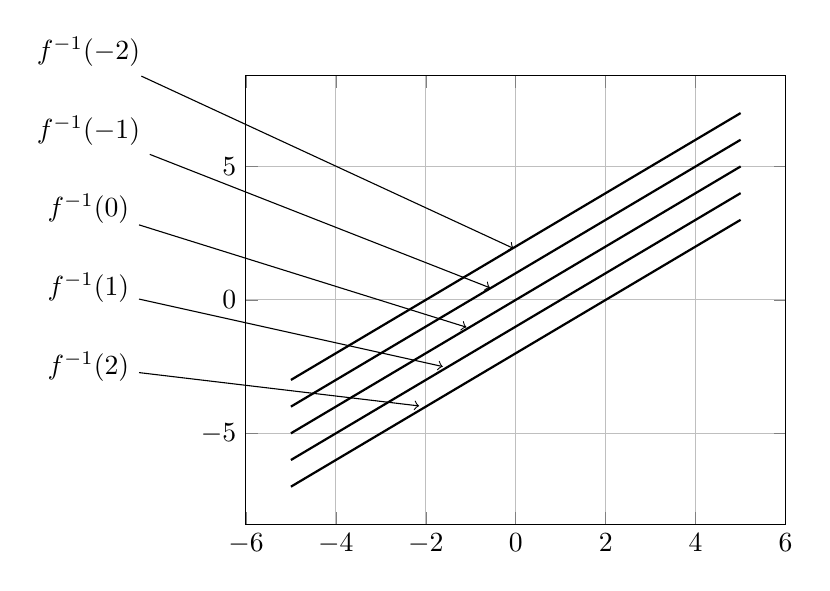
\begin{tikzpicture}
\begin{axis}[grid=both]
	\addplot[smooth,thick,black] {x-2};
	\addplot[smooth,thick,black] {x-1};
	\addplot[smooth,thick,black] {x-0};
	\addplot[smooth,thick,black] {x+1};
	\addplot[smooth,thick,black] {x+2};
\end{axis}
	\draw (-2,6) node(fm2){$f^{-1}(-2)$};
	\draw (-2,5) node(fm1){$f^{-1}(-1)$};
	\draw (-2,4) node(f0){$f^{-1}(0)$};
	\draw (-2,3) node(f1){$f^{-1}(1)$};
	\draw (-2,2) node(f2){$f^{-1}(2)$};

	\draw[->] (fm2) -- (3.4,3.5);
	\draw[->] (fm1) -- (3.1,3);
	\draw[->] (f0) -- (2.8,2.5);
	\draw[->] (f1) -- (2.5,2);
	\draw[->] (f2) -- (2.2,1.5);
\end{tikzpicture}
}
\caption{Level Set for $f(x_1,x_2) = x_1-x_2$}
\end{subfigure}
\hfill
\begin{subfigure}[t]{0.4\textwidth}
\centering
\scalebox{0.5}{
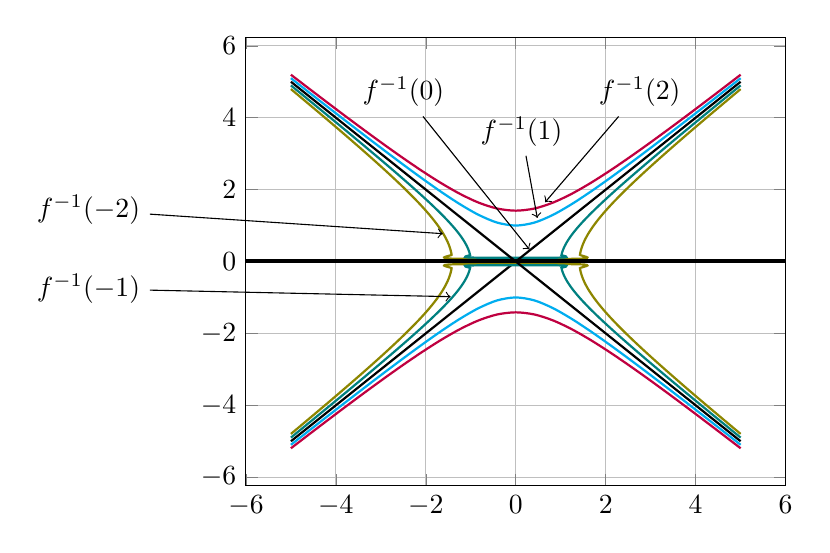
\begin{tikzpicture}
\begin{axis}[grid=both]
	\addplot[smooth,thick,olive,samples=1000] {sqrt(x^2-2)};
	\addplot[smooth,thick,teal,samples=1000] {sqrt(x^2-1)};
	\addplot[smooth,thick,black] {x};
	\addplot[smooth,thick,cyan] {sqrt(x^2+1)};
	\addplot[smooth,thick,purple] {sqrt(x^2+2)};

	\addplot[smooth,thick,olive,samples=1000] {-sqrt(x^2-2)};
	\addplot[smooth,thick,teal,samples=1000] {-sqrt(x^2-1)};
	\addplot[smooth,thick,black] {-x};
	\addplot[smooth,thick,cyan] {-sqrt(x^2+1)};
	\addplot[smooth,thick,purple] {-sqrt(x^2+2)};
\end{axis}

	\draw (-2,3.5) node(fm2){$f^{-1}(-2)$};
	\draw (-2,2.5) node(fm1){$f^{-1}(-1)$};
	\draw (2,5) node(f0){$f^{-1}(0)$};
	\draw (3.5,4.5) node(f1){$f^{-1}(1)$};
	\draw (5,5) node(f2){$f^{-1}(2)$};

	\draw[->] (fm2) -- (2.5,3.2);
	\draw[->] (fm1) -- (2.6,2.4);
	\draw[->] (f0) -- (3.6,3);
	\draw[->] (f1) -- (3.7,3.4);
	\draw[->] (f2) -- (3.8,3.6);

	\draw[ultra thick,black] (0,2.85)--(6.85,2.85);
\end{tikzpicture}
}
\caption{Level Set for $f(x_1,x_2) = x_1^2-x_2^2$}
\end{subfigure}
\end{figure}
In exercise 1.5-1.9, sketch the level sets of $f^{-1}(c)$ for $n=0,1$ and $2$ of each function at the heights indicated
\begin{enumerate} 
	\setcounter{enumi}{4}
	\item $f(x_1,x_2,\dots,x_{n+1}) = x_{n+1};\ c = -1,0,1,2$
	\item $f(x_1,x_2,\dots,x_{n+1}) = 0x_1^2 + x_2^2 + \dotsb + x_{n+1}^2;\ c = 0,1,4$
	\item $f(x_1,x_2,\dots,x_{n+1}) = x_1 - x_2^2 -\dotsb - x_{n+1}^2;\ c = -1,0,1,2$
	\item $f(x_1,x_2,\dots,x_{n+1}) = x_1^2 - x_2^2 - \dotsb - x_{n+1}^2;\ c = -1,0,1$
	\item $f(x_1,x_2,\dots,x_{n+1}) = x_1^2 + x_2^2/4 + \dotsb + x_{n+1}^2/(n+1)^2;\ c = 1$
	\item Show that graph of any function $f : \mathbb{R} \to \mathbb{R}$ is a level set for some function $F : \mathbb{R}^{n+1} \to \mathbb{R}$.\\

	\textbf{Solution : }
	Let $f : \mathbb{R}^n \to \mathbb{R}$ and $F : \mathbb{R}^{n+1} \to \mathbb{R}$ such that 
	$$F(x_1,x_2,\dots,x_{n+1}) = x_{n+1}-f(x_1,x_2,\dots,x_n)$$
	Then, $F^{-1}(0) = graph(f)$.
%	\begin{align*}
%		F^{-1}(0) & = \{ (x_1,x_2,\dots,x_{n+1}) : F(x_1,x_2,\dots,x_{n+1}) = 0 \} \\
%		& = \{ (x_1,x_2,\dots,x_n,x_{n+1}) : x_{n+1} - f(x_1,x_2,\dots,x_n) = 0 \}\\
%		& = \{ (x_1,x_2,\dots,x_n,x_{n+1}) : x_{n+1} = f(x_1,x_2,\dots,x_n) \}\\
%		& = graph(f)
%	\end{align*}
\end{enumerate}

%\chapter{Vector Fields}
\section{Vector Fields}
\begin{definition}
	A vector $\boldsymbol{v}$ at a point $p \in \mathbb{R}^{n+1}$ is a pair $\boldsymbol{v} = (p,v)$ where $v \in \mathbb{R}^{n+1}$.
\end{definition}
\begin{description}
	\item[vector addition] $\boldsymbol{v} + \boldsymbol{w} = (p,v) + (p,w) = (p,v+w)$.
	\item[scalar multiplication] Let $c \in \mathbb{R}$, then $c \boldsymbol{v} =  c(p,v) = (p,cv)$.
	\item[dot product] $\boldsymbol{v}\cdot \boldsymbol{w} = (p,v)\cdot(p,w) = v \cdot w$
	\item[cross product] $\boldsymbol{v}\times \boldsymbol{w} = (p,v)\times(p,w) = (p,v \times w)$
\end{description}
\begin{remark}
	Angle $\theta$ between $\boldsymbol{v}$ and $\boldsymbol{w}$ is given by,
	\begin{equation}
		\cos \theta = \boldsymbol{v}\cdot\boldsymbol{w} = (p,v)\cdot(p,w) = v.w
	\end{equation}
	And the length of a vector $\boldsymbol{v}$ is given by,
	\begin{equation}
		\|\boldsymbol{v}\| = \boldsymbol{v}\cdot\boldsymbol{v} = (p,v)\cdot(p,v) = v\cdot v = \| v \|
	\end{equation}
\end{remark}

\begin{remark}
	Let $c \in \mathbb{R}$ and $p \in \mathbb{R}^{n+1}$.
	Let $\boldsymbol{v}, \boldsymbol{w}$ be two vectors at $p$.
	That is, $\boldsymbol{v} = (p,v)$ and $\boldsymbol{w} = (p,w)$ for some $v,w \in \mathbb{R}^{n+1}$.
	Then \textbf{the set of all vectors at $p$ is a vector space} with vector addition $\boldsymbol{v}+\boldsymbol{w} = (p,v+w)$ and scalar multiplication $c\boldsymbol{v} = (p,cv)$.
	This vector space is denoted by $\mathbb{R}_p^{n+1}$.
\end{remark}

\begin{figure}[h]
	\centering
	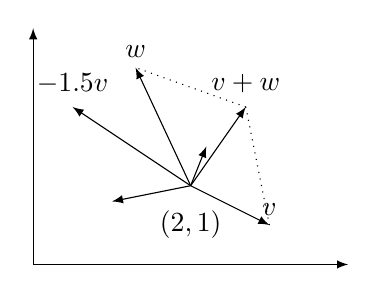
\begin{tikzpicture}
		\draw[-latex] (0,0) -- (0,3);
		\draw[-latex] (0,0) -- (4,0);

		\draw[-latex] (2,1) -- (1,0.8);
		\draw[-latex] (2,1) -- (2.2,1.5);
		%\draw[-latex] (2,1) -- (3,1.25);
		\draw[-latex] (2,1) -- (1.3,2.5); %w
		\draw[-latex] (2,1) -- (3,0.5); %v
		\draw[-latex] (2,1) -- (2.7,2); %v+w
		\draw[-latex] (2,1) -- (0.5,2); %1.5v
		\draw[dotted,thin] (3,0.5) -- (2.7,2);
		\draw[dotted,thin] (2.7,2)-- (1.3,2.5);

		\draw (2,0.5) node{$(2,1)$};
		\draw (3,0.7) node{$\boldsymbol{v}$};
		\draw (1.3,2.7) node{$\boldsymbol{w}$};
		\draw (2.7,2.3) node{$\boldsymbol{v+w}$};
		\draw (0.5,2.3) node{$-1.5\boldsymbol{v}$};
	\end{tikzpicture}
	\caption{The vector space of all vectors at $(2,1)$, $\mathbb{R}_{(2,1)}^2$}
\end{figure}

\begin{definition}
	The vector field $\boldsymbol{X}$ on $\mathbb{R}^{n+1}$ is a function which assigns to each point of $\mathbb{R}^{n+1}$ a vector at that point.
	That is, $\boldsymbol{X}(p) = (p,X(p))$.
\end{definition}

For example, $\boldsymbol{X}(p) = (p,X(p))$ where the associated function of the vector field, $X : \mathbb{R}^2 \to \mathbb{R}^2$ defined by $X(p) = (1,2)$ assigns a constant vector $(1,2)$ at every vector in $\mathbb{R}^2$.

\begin{figure}[h]
	\centering
	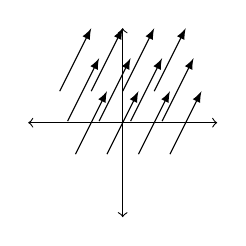
\begin{tikzpicture}[scale=0.4]
		\draw[<->] (-3,0) -- (3,0);
		\draw[<->] (0,-3) -- (0,3);

		\draw[-latex] (1,1) -- (2,3);
		\draw[-latex] (0,1) -- (1,3);
		\draw[-latex] (-1,1) -- (0,3);
		\draw[-latex] (-2,1) -- (-1,3);

		\draw[-latex] (1.25,0.05) -- (2.25,2.05);
		\draw[-latex] (0.25,0.05) -- (1.25,2.05);
		\draw[-latex] (-0.75,0.05) -- (0.25,2.05);
		\draw[-latex] (-1.75,0.05) -- (-0.75,2.05);

		\draw[-latex] (1.5,-1) -- (2.5,1);
		\draw[-latex] (0.5,-1) -- (1.5,1);
		\draw[-latex] (-0.5,-1) -- (0.5,1);
		\draw[-latex] (-1.5,-1) -- (-0.5,1);

	\end{tikzpicture}
	\caption{Vector field with associated function $X(p) = (1,2)$}
\end{figure}

\begin{definition}[smooth]
	A function $f : \mathbb{R} \to \mathbb{R}$ is smooth if its partial derivatives of all orders exists and are continuous.
	A function $f : \mathbb{R}^{n+1} \to \mathbb{R}$ is smooth if its component functions $f = (f_1, f_2, \dots, f_{n+1})$ are smooth.
	A vector field $\boldsymbol{X}$ is smooth if the associated function $X(p)$ is smooth.
\end{definition}

\begin{definition}
	Let $f : \mathbb{R}^{n+1} \to \mathbb{R}$. Then the gradient of $f$ at $p$ is,
	\begin{equation}
		\nabla f(p) = \left(p,\frac{\partial f}{\partial x_1}(p),\frac{\partial f}{\partial x_2}(p),\dots,\frac{\partial f}{\partial x_{n+1}}(p)\right)
	\end{equation}
\end{definition}

\begin{remark}
	If $f$ is a smooth function, then the gradient of $f$ at $p$ is a smooth vector field.
\end{remark}
	For example, $f : \mathbb{R}^2 \to \mathbb{R}$ defined by $f(x_1,x_2) = 2x_1x_2$ is a smooth function.
	We have, $\frac{\partial f}{\partial x_1} = 2x_2$ and $\frac{\partial f}{\partial x_2} = 2x_1$.
	And gradient of $f$ at $(x_1,x_2)$ is $(x_1,x_2,2x_2,2x_1)$.
	That is, $(2x_2,2x_1)$ at $(x_1,x_2)$.

Calculations : \\
\begin{tabular}{|c|c|c|c|c|c|c|} \hline
	$p$    & $(x_1,x_2)$   & $(0,0)$ & $(1,0)$ & $(0,1)$ & $(-1,0)$ & $(0,-1)$ \\ \hline
	$X(p)$ & $(2x_2,2x_1)$ & $(0,0)$ & $(0,2)$ & $(2,0)$ & $(0,-2)$ & $(-2,0)$ \\ \hline
\end{tabular}

\begin{figure}[h]
	\centering
	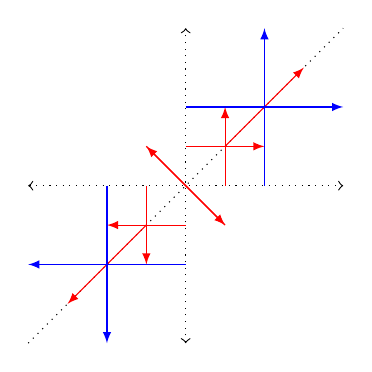
\begin{tikzpicture}[scale=0.5]
		\draw[<->,dotted] (0,-4) -- (0,4);
		\draw[<->,dotted] (-4,0) -- (4,0);
		\draw[dotted] (-4,-4) -- (4,4);

		\draw[-latex,color=red] (1,1) -- (3,3);
		\draw[-latex,color=red] (-1,1) -- (1,-1);
		\draw[-latex,color=red] (1,-1) -- (-1,1);
		\draw[-latex,color=red] (-1,-1) -- (-3,-3);
		\draw[-latex,color=red] (0,1) -- (2,1);
		\draw[-latex,color=red] (0,-1) -- (-2,-1);
		\draw[-latex,color=red] (1,0) -- (1,2);
		\draw[-latex,color=red] (-1,0) -- (-1,-2);

		%\draw[-latex] (-1,2) -- (3,0);
		%\draw[-latex] (2,-1) -- (0,3);
		%\draw[-latex] (1,-2) -- (-3,0);
		%\draw[-latex] (-2,1) -- (0,-3);

		\draw[-latex,color=blue] (0,2) -- (4,2);
		\draw[-latex,color=blue] (2,0) -- (2,4);
		\draw[-latex,color=blue] (-2,0) -- (-2,-4);
		\draw[-latex,color=blue] (0,-2) -- (-4,-2);

		%\draw[-latex] (1,0.5) -- (2,2.5);
		%\draw[-latex] (0.5,1) -- (2.5,2);
		%\draw[-latex] (-1,0.5) -- (0,-1.5);
		%\draw[-latex] (0.5,-1) -- (-1.5,0);
		%\draw[-latex] (1,-0.5) -- (0,1.5);
		%\draw[-latex] (-0.5,1) -- (1.5,0);
		%\draw[-latex] (-1,-0.5) -- (-2,-2.5);
		%\draw[-latex] (-0.5,-1) -- (-2.5,-2);
	\end{tikzpicture}
	\caption{The gradient of $f(x_1,x_2) = 2x_1x_2$}
\end{figure}

\begin{definition}
	A parameterised curve is a function, $\alpha : I \to \mathbb{R}^{n+1}$ where $I$ is some open interval in $\mathbb{R}$.
	The velocity vector of a parameterised curve $\alpha : I \to \mathbb{R}^{n+1}$ at a point $\alpha(t)$ is the tangent to the curve at that point.
	\begin{equation}
		\dot{\boldsymbol{\alpha}}(t) = \left(\alpha(t),\frac{d \alpha}{dt} (t)\right)
	\end{equation}
\end{definition}

For example, $\alpha : I \to \mathbb{R}^2$ defined by $\alpha(t) = (2t,t^2)$ is a parameterised curve.
We have, $\frac{d\alpha}{dt} = (\frac{dx_1}{dt}(t),\frac{dx_2}{dt}(t)) = (2,2t)$ where $\alpha(t) = (x_1(t),x_2(t))$.
The velocity vector at $t = 3$ is $\dot{\alpha}(3) = (\alpha(t),\frac{d\alpha}{dt}) = (6,9,2,6)$.

\begin{definition}
	Let $\boldsymbol{X}$ be a vector field and let $U$ be an open subet of $\mathbb{R}^{n+1}$.
	An integral curve $\alpha$ on $U$ is a parameterised curve, $\alpha : I \to \mathbb{R}^{n+1}$ such that for each $\alpha(t) = p \in U$, the velocity vector $\dot{\alpha}(t)$ is the associated vector $\boldsymbol{X}(p)$ of the vector field $\boldsymbol{X}$ at that point.
	Thus, for each $t \in I$, $\dot{\alpha}(t) = \boldsymbol{X}(\alpha(t))$.
	\begin{equation}
		\left(\alpha(t),\frac{d \alpha}{dt}(t)\right) = \left(\alpha(t),X(\alpha(t))\right)
	\end{equation}
	Let $X(p) = \left(X_1(p),X_2(p),\dots,X_{n+1}(p)\right)$ and $\alpha(t) = \left(x_1(t),x_2(t),\dots,x_{n+1}(t)\right)$.
	Then, comparing components of the vector at $\alpha(t)$ we get the following system of equations,
	\begin{equation}
		\frac{d x_j}{dt}(t) = X_j(\alpha(t)),\ j = 1,2,\dots,(n+1)
	\end{equation}
\end{definition}

For example, Consider $\alpha : (2,3) \to \mathbb{R}^2$ defined by $\alpha(t) = (t,t^2)$.
Then $\alpha$ is a parameterised curve in vector field, $\boldsymbol{X}$ which has the associated function $X(x_1,x_2) = (1,2x_1)$.
Then, $\boldsymbol{X}(x_1,x_2) = (x_1,x_2,1,2x_1)$.
And
\[ \dot{\alpha}(t) = \left( \alpha(t),\frac{d\alpha}{dt}(t) \right) = \left( x_1(t),x_2(t),\frac{dx_1}{dt}(t), \frac{dx_2}{dt}(t) \right) = (t,t^2,1,2t) \]
Clearly, $\alpha$ is an integral curve of $\boldsymbol{X}$ as $\dot{\alpha}(t) = X(\alpha(t))$ for every $t \in (2,3)$.

Calculations:\\
\begin{tabular}{|c|c|c|c|c|c|c|c|c|c|} \hline
	$p$    & $(0,0)$ & $(1,0)$ & $(0,1)$ & $(1,1)$ & $(-1,0)$ & $(0,-1)$ & $(-1,1)$ & $(1,-1)$ & $(-1,-1)$ \\ \hline
	$X(p)$ & $(1,0)$ & $(2,2)$ & $(1,1)$ & $(2,3)$ & $(0,-2)$ & $(1, 1)$ & $(0,-1)$ & $(2, 1)$ & $( 0,-3)$ \\ \hline
\end{tabular}

\begin{figure}[h]
	\centering
	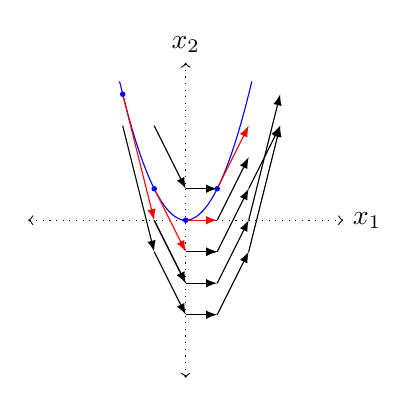
\begin{tikzpicture}[scale=0.4]
		\draw[<->,dotted] (-5, 0) -- (5, 0) node[right] {$x_1$};
  		\draw[<->,dotted] (0,-5) -- (0, 5) node[above] {$x_2$};
  		\draw[domain=-2.1:2.1, smooth, variable=\x, blue] plot ({\x}, {\x*\x});

		\draw[-latex,color=red] (0,0) -- (1,0);

		\draw[-latex] (0,1) -- (1,1);
		\draw[-latex] (1,0) -- (2,2);
		\draw[-latex] (-1,3) -- (0,1);

		\draw[-latex,color=red] (-2,4) -- (-1,0);
		\draw[-latex,color=red] (1,1) -- (2,3);

		\draw[-latex] (0,-1) -- (1,-1);
		\draw[-latex,color=red] (-1,1) -- (0,-1);

		\draw[-latex] (-1,0) -- (0,-2);
		\draw[-latex] (0,-2) -- (1,-2);
		\draw[-latex] (1,-2) -- (2,0);
		\draw[-latex] (2,0) -- (3,4);

		\draw[-latex] (0,-1) -- (1,-1);
		\draw[-latex] (-1,0) -- (0,-2);

		\draw[-latex] (-2,3) -- (-1,-1);
		\draw[-latex] (-1,-1) -- (0,-3);
		\draw[-latex] (0,-3) -- (1,-3);
		\draw[-latex] (1,-3) -- (2,-1);
		\draw[-latex] (2,-1) -- (3,3);

		\draw[-latex] (0,-1) -- (1,-1);
		\draw[-latex] (1,-1) -- (2,1);
		\draw[-latex] (2,1) -- (3,3);

		\node[circle,fill=blue,inner sep=0pt, minimum size=2pt] at (1,1){};
		\node[circle,fill=blue,inner sep=0pt, minimum size=2pt] at (0,0){};
		\node[circle,fill=blue,inner sep=0pt, minimum size=2pt] at (-1,1){};
		\node[circle,fill=blue,inner sep=0pt, minimum size=2pt] at (-2,4){};
\end{tikzpicture}
	\caption{Integral Curve $\alpha(t) = (t,t^2)$ in $\boldsymbol{X}$ with $X(x_1,x_2) = (1,2x_1)$}
\end{figure}

\begin{theorem}
	Let $\boldsymbol{X}$ be a smooth vector field on an open set $U \subset \mathbb{R}^{n+1}$ and let $p \in U$.
	Then there exists an open interval $I$ containing $0$ and an integral curve $\alpha : I \to U$ such that
	\begin{enumerate}
		\item $\alpha(0) = p$
		\item If $\beta : \tilde{I} \to U$ is any other integral curve with $\beta(0) = p$, then $\tilde{I} \subset I$ and $\beta(t) = \alpha(t)$, for all $t \in \tilde{I}$.
	\end{enumerate}
\end{theorem}
\begin{proof}
	Let $\boldsymbol{X}$ be a smooth vector field.
	Suppose $\alpha$ be an integral curve in $\boldsymbol{X}$.
	Then, $\dot{\alpha}(t) = \boldsymbol{X}(\alpha(t))$.
	Let $x_j(t)$ be the components of $\alpha(t)$ and $X_j(p)$ be the components of $X(p)$.
	\begin{align*}
		\dot{\alpha}(t) & = \left(\alpha(t),\frac{d \alpha}{dt}(t)\right) \\
		& = \left(x_1(t),\dots,x_{n+1}(t),\frac{dx_1}{dt}(t),\dots,\frac{dx_{n+1}}{dt}(t)\right)\\
		\boldsymbol{X}(\alpha(t)) & = (\alpha(t),X(\alpha(t))) \\
		& = \left( x_1(t),\dots,x_{n+1}(t),X_1(\alpha(t)),\dots,X_{n+1}(\alpha(t))\right)
	\end{align*}
	Thus, we a system of $n+1$ first order differential equations in $n+1$ unknowns satisfying the initial condition $\alpha(0) = p$.
	\begin{align*}
		\frac{dx_1}{dt}(t) & = X_1(\alpha(t)) \\
		\frac{dx_2}{dt}(t) & = X_2(\alpha(t)) \\
		& \vdots \\
		\frac{dx_{n+1}}{dt}(t) & = X_{n+1}(\alpha(t))
	\end{align*}
\end{proof}
	By the theorem on solution of systems of first order ordinary differential equations, there exists an interval $I$ containing $0$ and a solution --- a family of functions $\{ x_1(t), x_2(t), \dots,x_{n+1}(t)\}$ satisfying the above system of equations satisfying the initial condition $\alpha(0) = p$.

	Define $\alpha : I \to U$ using the component functions of $\alpha$ as $x_j$s in the above solution.
	Then, we have a integral curve of the vector field $\boldsymbol{X}$ satifying the initial condition $\alpha(0) = p$.

	Let $\beta : \tilde{I} \to U$ be another integral curve with $\beta(0) = p$.
	Then by the uniqueness of the solution for the system of first order ordinary differential equations with an initial condition, $\beta(t) = \alpha(t)$ for every $ t \in I \cup \tilde{I}$.

	Let $\{\beta_1,\beta_2,\dots\}$ be the family of integral curves with $\beta_j : I_j \to U$ satisfying $\beta_j(0) = p$.
	Consider $I = \bigcup\limits_{j \in \mathbb{N}} I_j$.

	Define $\alpha : I \to U$ by $\alpha(t) = \beta_j(t)$ where $t \in I_j$ for some $j \in \mathbb{N}$.
	Then $\alpha$ is well-defined and is a maximal integral curve in $\boldsymbol{X}$ such that $\alpha(0) = p$.

\begin{definition}
	A smooth vector field $\boldsymbol{X}$ on $U \subset \mathbb{R}^{n+1}$ is \textbf{complete} if for every $p \in U$, the maximal integral curve through $p$ has domain equal to $\mathbb{R}$.
\end{definition}

\begin{definition}
	The \textbf{divergence} of a smooth vector field $\boldsymbol{X}$ on $U \subset \mathbb{R}^{n+1}$ is the function $div\ \boldsymbol{X} : U \to \mathbb{R}$ defined by
	\[ div\ X(x_1,x_2,\dots,x_{n+1}) = \sum_{i=1}^{n+1} \frac{\partial X_i}{\partial x_i} \]
	where $X_i$ are the component function of the associated function $X$ of the vector field $\boldsymbol{X}$.
\end{definition}

For example, Consider $\boldsymbol{X}$ with associated function $X : \mathbb{R}^2 \to \mathbb{R}^2$ defined by $X(x_1,x_2) = (2x_1,x_1x_2)$.
Then $div\ \boldsymbol{X}(x_1,x_2) = \frac{\partial X_1}{\partial x_1} + \frac{\partial X_2}{\partial x_2} = 2 + x_1$.

%\chapter{The Tangent Space}
\section{The Tangent Space}
\begin{definition}
	Let $f:U \to \mathbb{R}$ be a smooth function.
	Suppose $f^{-1}(c)$ is nonempty and $p \in f^{-1}(c)$.
	A vector $\boldsymbol{v}$ is a \textbf{vector tangent to $f^{-1}(c)$ at $p$} if there exists a parametrized curve $\alpha : I \to U$ such that $\alpha$ is contained in $U$, $\alpha(0) = p$ and $\dot\alpha(0) = \boldsymbol{v}$.
\end{definition}

\begin{lemma}
	The gradient of $f$ at $p \in f^{-1}(c)$ is orthogonal to all vectors tangent to $f^{-1}(c)$ at $p$.
\end{lemma}
\begin{proof}
\begin{align*}
	f \circ \alpha(t) & = f(x_1(t),x_2(t),\dots,x_{n+1}(t))\\
	\frac{d f \circ \alpha(t)}{dt}
	& = \frac{\partial f}{\partial x_1} \frac{d}{dt}x_1(t) + \frac{\partial f}{\partial x_2} \frac{d}{dt}x_2(t)+\dots + \frac{\partial f}{\partial x_{n+1}} \frac{d}{dt}x_{n+1}(t) \\
	& = \left( \frac{\partial f(\alpha(t_0))}{\partial x_1},\frac{\partial f(\alpha(t_0))}{\partial x_2},\dots,\frac{\partial f(\alpha(t_0))}{\partial x_{n+1}} \right) \cdot \left( \frac{dx_1(t)}{dt} , \frac{dx_2(t)}{dt} ,\dots,\frac{dx_{n+1}(t)}{dt} \right) \\
	& = (\nabla f)(\alpha(t_0)) \cdot \dot\alpha(t_0)
\end{align*}
	Clearly, $f \circ \alpha(t_0) = c$ and $\frac{d}{dt} f \circ \alpha(t_0) = \nabla f(\alpha(t_0)) \cdot \dot\alpha(t_0) = 0$.
	Since parametrized curve $\alpha$ is arbitrary, the gradient vector $\nabla f(\alpha(t_0))$ is orthogonal to every vector tangent to $f^{-1}(c)$ at $\alpha(t_0)=p$.
\end{proof}

\begin{theorem}
	Let $U$ be an open set, $f : U \to \mathbb{R}$ be a smooth function and $p \in U$ be a regular point of $f$.
	If $f(p)=c$, then the set all vectors tangent to $f^{-1}(c)$ at $p$ is equal to $[\nabla f(p)]^\perp$.
\end{theorem}
\begin{proof}
	A vector $\boldsymbol{v}$ is tangent to $f^{-1}(c)$ at $p$ if there exists a parametrised curve $\alpha$ on $f^{-1}(c)$ such that $\alpha(0) = p$ and $\dot\alpha(0)=v$.  We know that $f(p) = c$. By chain rule, $f'(p) = \nabla f(\alpha(0)) \cdot \dot\alpha(0) = \nabla f(p) \cdot v = 0$. Clearly, $\boldsymbol{v} \in [\nabla f(p)]^\perp$.\\

	It is enough to prove that if $\boldsymbol{v} = (p,v) \in [\nabla f(p)]^\perp$ then there exists a parametrized curve $\alpha$ contained in $f^{-1}(c)$ which passes through $p$ and has tangent vector $v$ at $p$.\\

	Let $\boldsymbol{v} = (p,v) \in [\nabla f(p)]^\perp$. Consider constant vector field $\boldsymbol{X}$ on $U$ defined by, $\boldsymbol{X}(q) = (q,v)$. Consider another vector field $\boldsymbol{Y}$ defined by subtracting the component of $\boldsymbol{X}$ along $\nabla f(q)$.
	$$\boldsymbol{Y}(q) = \boldsymbol{X}(q) - \frac{\boldsymbol{X}(q) \cdot \nabla f(q)}{\| \nabla f(q) \|^2} \nabla f(q)$$
	The domain of $\boldsymbol{Y}$ is the open subset of $U$ such that $\nabla f(q) \ne 0$. Since $p$ is a regular point of $f$, $p$ is in the domain of $\boldsymbol{Y}$. And $\boldsymbol{Y}(p) = \boldsymbol{X}(p)$ since $\boldsymbol{X}(p) \cdot \nabla f(p) = 0$. By construction, $\boldsymbol{Y}$ is a smooth vector field orthogonal to $\nabla f(q)$ for every point $q$ in its domain and $\boldsymbol{Y}(p) = \boldsymbol{v}$.\\

	Since $Y$ is smooth vector field defined on an open set, there exists a maximal integral curve through $p$, say $\alpha$. Thus, $\alpha : I \to \mathscr{D}(Y)$ such that $\dot\alpha(t)=\boldsymbol{Y}(\alpha(t))$ and $\alpha(0)=p,\ 0 \in I$. Clearly, $\dot\alpha(0)=\boldsymbol{Y}(p) = \boldsymbol{v}$.
	\begin{align*}
		\frac{d}{dt} f(\alpha(t)) 
		& = \nabla f(\alpha(t)) \cdot \dot\alpha(t) \text{ by chain rule }\\
		& = \nabla f(\alpha(t)) \cdot \boldsymbol{Y}(\alpha(t)) \text{ since } \dot\alpha(t) = \boldsymbol{Y}(\alpha(t)) \\
		& = \boldsymbol{0} \text{ since }\boldsymbol{Y} \perp \nabla f(\alpha(t))
	\end{align*}
	Clearly, $f(\alpha(t))$ is a constant and $f(\alpha(0)) = f(p) = c$ since $p \in f^{-1}(c)$. Therefore, $f(\alpha(t)) = c,\ \forall t \in I$. Clearly, $\alpha$ is contained in $f^{-1}(c)$. Therefore, there exists a parametrized curve $\alpha$ such that $\dot\alpha(0) = \boldsymbol{v}$. Since $\boldsymbol{v}$ is arbitrary, every vector orthogonal to $\nabla f(p)$ is a tangent vector to $f^{-1}(c)$ at $p$.
\end{proof}

\begin{definition}
	Let $S$ be an $n$-surface and $p \in S$.
	The set of all vector tangent to $S$ at $p$ is called the \textbf{tangent space} $S_p$.
	If $p$ is a regular point of $f$ and $f(p) = c$. Then the \textbf{tangent space} $S_p$ of the surface $S = f^{-1}(c)$ at $p$ is spanned by the vector $\nabla f(p)$.
	That is, $S_p = [\nabla f(p)]^\perp$.
\end{definition}

%\chapter{Surfaces}
\section{Surfaces}
\begin{definition}
	A \textbf{surface} of dimension $n$, or $n$-surface in $\mathbb{R}^{n+1}$ is a nonempty subset of the form $S = f^{-1}(c)$ where $f : U \to \mathbb{R}$ such that $U$ is an open subset of $\mathbb{R}^{n+1}$, $f$ is a smooth function  and $\nabla f(p) \ne 0,\ \forall p \in S$.
\end{definition}
	The $n$-surfaces are usually called \textbf{plane curves}, \textbf{surfaces} or \textbf{hypersurfaces} when $n=1$, $n=2$ and $n>2$ respectively.

\begin{remark}
	Let $S$ be an $n$-surface and $p \in S$.
	Then it has the tangent space $S_p$ which is an $n$ dimensional subspace of the vector space $\mathbb{R}_p^{n+1}$.\\

	It is important to note that, the tangent space $S_p$ depends on the surface $S$, the point $p$ and is independent of the the function $f$.
\end{remark}

\begin{definition}
	The \textbf{$n$-sphere} $S^n$ is the level set $f^{-1}$ where $f : \mathbb{R}^{n+1} \to \mathbb{R}$ defined by $f(x_1,x_2,\dots,x_{n+1}) = x_1^2+x_2^2+\dots+x_{n+1}^2$.
\end{definition}
	The $1$-sphere, $S^1$ is the unit circle.

\begin{definition}
	The \textbf{$n$-plane} is the level set $f^{-1}(c)$ where $f : \mathbb{R}^{n+1} \to \mathbb{R}$ defined by $f(x_1,x_2,\dots,x_{n+1}) = a_1x_1+a_2x_2+\dots+a_{n+1}x_{n+1}$.
\end{definition}
	We may express $f(x) = a \cdot x$ where $a,x \in \mathbb{R}^{n+1}$.
	The $n$-planes are \textbf{lines}, \textbf{planes} and \textbf{hyperplanes} when $n=1$, $n=2$ and $n>2$ respectively.

\begin{definition}
	Let $S$ be an $(n-1)$-surface.
	Then $S = f^{-1}(c)$ for some function $f : \mathbb{R}^n \to \mathbb{R}$.
	The \textbf{cylinder over the surface $S$} is the $n$-surface $g^{-1}(c)$ where $g(x_1,x_2,\dots,x_{n+1}) = f(x_1,x_2,\dots,x_n)$.
\end{definition}

\begin{commentary}
	In general, let $S = f^{-1}(c)$ where $f : U \to \mathbb{R}$. Then the cylinder over S is an $n$-surface given by $g^{-1}(c)$ where $g : U \times \mathbb{R} \to \mathbb{R}$ defined by $g(\boldsymbol{u},t) = f(\boldsymbol{u})$ where $u \in U,\ t \in \mathbb{R}$.\\
	
	The name comes from the cylinder over the unit circle.
\end{commentary}

\begin{definition}
	Let $C$ be a curve in $\mathbb{R}^2$ which lies above $x_1$ axis. Then $C = f^{-1}(c)$ where $f : U \to \mathbb{R}$, $\nabla f(p) \ne 0,\ p \in C$ and $U$ is contained in the upper half plane $x_2 > 0$.
	Then \textbf{surface of revolution obtained by rotating $C$ about the $x_1$ axis} is given $S = g^{-1}(c)$ where $g(x_1,x_2,x_3) = f(x_1,(x_2^2+x_3^2)^\frac{1}{2})$.
\end{definition}

\begin{theorem}[Lagrange`s Multiplier]
	Let $S$ be an $n$-surface in $\mathbb{R}^{n+1}$, $S = f^{-1}(c)$ where $f : U \to \mathbb{R}$ is such that $\nabla f(q) \ne 0,\ \forall q \in S$. Suppose $g : U \to \mathbb{R}$ is a smooth function and $p \in S$ is an extreme point of $g$ on $S$. Then there exists a real number $\lambda$ such that $\nabla g(p) = \lambda \nabla f(p)$.
\end{theorem}
\begin{proof}
	Let $S$ be an $n$-surface with $p \in S$ as an extreme point of smooth function $g$ on $S$.
	We know that, $S_p = [\nabla f(p)]^\perp$.
	Clearly, $S_p^\perp$ is $1$-dimensional in $\mathbb{R}^{n+1}$ spanned by $\nabla f(p) \ne 0$.\\

	Let $\boldsymbol{v} \in S_p$. Then there exists a parametrized curve $\alpha$ on $S$ such that $\alpha(0) = p$ and $\dot\alpha(0) = \boldsymbol{v}$.
	Clearly, $g'(\alpha(0)) = g'(p) = 0$ since $p$ is an extreme point of $g$ on $S$.
	$$ g'(\alpha(0)) = \nabla g(\alpha(0)) \cdot \dot\alpha(0) = \nabla g(p) \cdot \boldsymbol{v} = 0 $$
	Thus, $\nabla g(p) \in S_p^\perp$.
	Therefore, $\nabla g(p) = \lambda \nabla f(p)$.
\end{proof}

\begin{remark}
	Let $p$ be an extreme point of a smooth function $g$ defined on an $n$-surface $f^{-1}(c)$.
	The \textbf{Lagrange`s multiplier} $\lambda$ is a real number such that $\nabla g(p) = \lambda \nabla f(p)$.
	If $S$ is compact, then every smooth function on $S$ attains both minimum and maximum on $S$.
\end{remark}

\begin{important}
	The function $g(x_1,x_2) = ax_1^2 + 2bx_1x_2 + cx_2^2$ attains extrema on unit circle, $f^{-1}(1)$ where $f(x_1,x_2) = x_1^2 + x_2^2$. We know that 
	\begin{align*}
		\nabla f(x_1,x_2) & = (x_1,x_2,2x_1,2x_2) \text{ and } \\
		\nabla g(x_1,x_2) & = (x_1,x_2,2ax_1+2bx_2,2bx_1+2cx_2)
	\end{align*}
	By Lagrange`s multiplier theorem, $\nabla g(x_1,x_2) = \lambda \nabla f(x_1,x_2)$. Thus,
	\begin{align*}
		2ax_1 +2bx_2 & = 2\lambda x_1 \\
		2bx_1 +2cx_2 & = 2\lambda x_2 
	\end{align*}
	We may write, $\begin{pmatrix}a & b \\ b & c \end{pmatrix} \begin{pmatrix} x_1 \\ x_2 \end{pmatrix} = \lambda \begin{pmatrix} x_1 \\ x_2 \end{pmatrix} $.
	We know that, $\lambda$, $\begin{pmatrix}x_1 \\ x_2 \end{pmatrix}$  satisfying the condition are the eigenvalues and eigenvectors of the matrix $\begin{pmatrix} a & b \\ b & c \end{pmatrix}$ respectively. Clearly, the extreme points of the function $g$ are the eigenvectors of the matrix.
\end{important}

\subsection*{Exercise}
\begin{enumerate}
	\setcounter{enumi}{11}
	\item Show that the extreme values of the function $g(\boldsymbol{x}) = \sum_{i,j} a_{i,j} x_i x_j$ on the unit sphere $x_1^2 + x_2^2 + \dotsb + x_{n+1}^2 = 1$, where $(a_{i,j})$ is a symmetric matrix of real numbers, are eigen values of the matrix $(a_{i,j})$.
	\begin{important}
		\begin{align*}
			\nabla f(p) & = (p,2p) \\
			\nabla g(p) & = (p,2\sum_j a_{1,j}x_j,\dots,2\sum_j a_{n+1,j} x_j) 
		\end{align*}
		By Lagrange`s theorem, $\nabla g(p) = \lambda \nabla f(p)$. Thus,
		$$ \begin{pmatrix} a_{1,1} & a_{1,2} & \dots & a_{n+1,1} \\ a_{2,1} & a_{2,2} & \dots & a_{n+1,2} \\ \vdots & \vdots & \ddots & \vdots \\ a_{n+1,1} & a_{n+1,2} & \dots & a_{n+1,n+1} \end{pmatrix} \begin{pmatrix} x_1 \\ x_2 \\ \vdots \\ x_{n+1} \end{pmatrix} = \lambda \begin{pmatrix} x_1 \\ x_2 \\ \vdots \\ x_{n+1} \end{pmatrix}  $$
	Let $p = (p_1,p_2,\dots,p_{n+1})$. Then, $\|p\|^2 = 1$ since $p \in S^2$.
	$$ g(p) = [P][a_{i,j}][P]' = [P]\lambda[P]' = \lambda \|p\|^2 = \lambda $$
	We know that all eigenvalues of a real symmetric matrix is real. 
	Therefore, the minimum and maximum values of $g$ are the minimum and maximum eigenvalues of the matrix.
	\end{important}
	\setcounter{enumi}{14}
	\item Suppose $(x_1,x_2,x_3,x_4) \in \mathbb{R}^4$ is represented by $\begin{pmatrix} x_1 & x_2 \\ x_3 & x_4 \end{pmatrix}$. Then $SL(2,\mathbb{R})$ is a $3$-surface in $\mathbb{R}^4$.\\

\begin{important}
	Special Linear Group, $SL(2,\mathbb{R})$ is defined as the set of all $2 \times 2$ real matrices with determinant $1$. That is, $x_1x_4 - x_2x_3 = 1$. Consider the function $f : \mathbb{R}^4 \to \mathbb{R}$ defined by $f(x_1,x_2,x_3,x_4) = x_1x_4 - x_2x_3$. Then $SL(2,\mathbb{R})$ is nothing but $f^{-1}(1)$.\\

	We know that the domain of $f$ is open, $f$ is a smooth function and $\nabla f(x_1,x_2,x_3,x_4) = (x_1,x_2,x_3,x_4,x_4,-x_3,-x_2,x_1)$.
	Thus, $\nabla f(p) = 0$ if and only if $p = 0$. But $0 \notin SL(2,\mathbb{R})$. Therefore, $SL(2,\mathbb{R})$ is a $3$-surface.
\end{important}
\end{enumerate}

%\chapter{Vector Fields on Surfaces; Orientation}
\section{Vector Fields on Surfaces; Orientation}
\begin{definition}
	Let $S$ be an $n$-surface and $X$ be a smooth function defined $S$ such that $X(p) \in \mathbb{R}^{n+1},\ \forall p \in S$.
	Then $\boldsymbol{X}(p) = (p,X(p))$ is a \textbf{vector field on the $n$-surface} $S$.
\end{definition}
\begin{commentary}
	We know that $\nabla f(p) \ne 0,\ \forall p \in S$. Then there exists an open set $U$ containing $S$ such that $\nabla f(q) \ne 0,\ \forall q \in U$. The construction of $U$ is as follows, Let $p \in S$. Then $\nabla f(p) \ne 0$. Since $f$ is smooth, there exists a neighbourhood $P$ of $p$ in which $\nabla f(p) \ne 0$. Clearly $\displaystyle \bigcup_{p \in S} P$ is an open set containing $S$ in which $\nabla f(p) \ne 0$.
\end{commentary}

\begin{definition}
	A \textbf{tangent vector field $\boldsymbol{X}$ on an $n$-surface $S$} is a vector field on $S$ which assigns to each point $p \in S$ a vector tangent to $S$ at $p$.
	A \textbf{normal vector field $\boldsymbol{X}$ on an $n$-surface $S$} is a vector field on $S$ which assigns to each point $p \in S$ a vector orthogonal to $S$ at $p$.
\end{definition}

\begin{definition}
	A vector field $\boldsymbol{X}$ on an $n$-surface $S$ is \textbf{smooth} if $\boldsymbol{X}$ it is a restriction of a smooth vector field defined on an open set.
\end{definition}

\begin{theorem}[maximal integral curve on a surface]
	Let $S$ be an $n$-surface in $\mathbb{R}^{n+1}$, let $X$ be a smooth tangent vector field on $S$, and let $p \in S$. Then there exists an interval $I$ containing $0$ and a parametrized curve $\alpha : I \to S$ such that
	\begin{enumerate}
		\item $\alpha(0) = p$.
		\item $\dot\alpha(0) = \boldsymbol{X}(\alpha(t)),\ \forall t \in I$.
		\item If $\beta : \tilde{I} \to S$ is any other parametrized curve satisfying above conditions, then $\tilde{I} \subset I$ and $\beta(t) = \alpha(t),\ \forall t \in I \cap \tilde{I}$.
	\end{enumerate}
\end{theorem}
\begin{proof}
	Let $S$ be an $n$-surface. And $\boldsymbol{X}$ be a smooth tangent vector field on $S$. By the definition of smooth vector field, $\boldsymbol{X}$ should be a restriction of a smooth vector field $\tilde{\boldsymbol{X}}$ on an open set $V$ containing $S$. Let function $f : U \to \mathbb{R}$, $c \in \mathbb{R}$ such that $f^{-1}(c) = S$ and $\nabla f(q) \ne 0,\ \forall q \in S$. Let $W = \{ q \in U \cap V : \nabla f(q) \ne 0 \}$. Clearly $W$ is open.\footnote{$\{ q \in \mathbb{R}^{n+1} : \nabla f(q) \ne 0\}$ is an open in $\mathbb{R}^{n+1}$ since $\{ q \in \mathbb{R}^{n+1} : \nabla f(q) = 0 \}$ is closed.} And contains $S$. And $\tilde{\boldsymbol{X}}, f$ are defined on $W$. Consider the vector field $\boldsymbol{Y}$ on $W$ defined by
	$$ \boldsymbol{Y}(q) = \tilde{\boldsymbol{X}}(q) - \frac{\tilde{\boldsymbol{X}} \cdot \nabla f(q)}{\|\nabla f(q)\|^2} \nabla f(q) $$
	Then $\boldsymbol{Y}$ is a vector field on $W$ such that it is tangent to level set of $f$ since we have removed the components orthogonal to the level sets from each vector assigned.\\

	Clearly, $\boldsymbol{Y}(p) = \tilde{\boldsymbol{X}}(p),\ \forall p \in S$ since $\tilde{\boldsymbol{X}}(p) \cdot \nabla f(p) = 0$ for each $p \in S$.  We already know that, $\tilde{\boldsymbol{X}}(p) = \boldsymbol{X}(p),\ \forall p \in S$. Now $\boldsymbol{Y}$ is a smooth vector defined on an open set $W$.\\

	By maximal integral theorem, there exists a maximal integral on $\boldsymbol{Y}$ through $p$, say $\alpha : I \to W$.
	Then $(f \circ \alpha)'(t) = \nabla f(\alpha(t)) \cdot \dot\alpha(t) = \nabla f(\alpha(t)) \cdot \boldsymbol{Y}(\alpha(t)) = 0$, since $\boldsymbol{Y}$ is tangent to the level sets of $f$ by construction. Thus, $f(\alpha(t))$ is constant. However, $f(\alpha(0)) = f(p) = c$. Thus, $f(\alpha(t)) = c, \forall t \in I$. Therefore, $\alpha(t) \in f^{-1}(c) = S,\ \forall t \in I$. Clearly, $\alpha$ is contained in $S$. Now, we have an integral curve on $S$.\\

	Suppose $\beta : \tilde{I} : W$ be another integral curve on $W$ through $p$. Then $\alpha(t) = \beta(t),\ \forall t \in I \cap \tilde{I}$ by the uniqueness of the integral curve on $\boldsymbol{Y}$. Let $\{ \alpha_j : i \in I\}$ be the set of all integral curves on $\boldsymbol{Y}$ passing through $p$. Let $I$ be union of the domain of $\alpha_j$`s.  Clearly, $I$ is an interval containing $0$. Then $\alpha : I \to W$ is a maximal integral on $\boldsymbol{Y}$ passing through $p$ where $\alpha(t) = \alpha_j(t),\ t \in \mathscr{D}(\alpha_j)$.
\end{proof}

\begin{corollary}
	Let $S$ be an $n$-surface where $S = f^{-1}(c)$, $f : U \to \mathbb{R}$ and $\nabla f(q) \ne 0,\forall q \in S$. Let $\boldsymbol{X}$ be a smooth vector field on $U$ whose restriction to $S$ is a tangent vector field on $S$. If $\alpha : I \to U$ is an integral curve on $\boldsymbol{X}$ such that $\alpha(t_0) \in S$ for some $t_0 \in I$, then $\alpha(t) \in S,\ \forall t \in I$.
\end{corollary}
\begin{proof}
	%yet to complete
\end{proof}

\begin{theorem}[orientation]
	Let $S$ be a connected, $n$-surface. Then there exists on $S$ exactly two unit normal vector fields $\boldsymbol{N}_1$ and $\boldsymbol{N}_2$, and $\boldsymbol{N}_1(p) = -\boldsymbol{N}_2(p),\ \forall p \in S$.
\end{theorem}
\begin{proof}
	%yet to complete
\end{proof}

\begin{definition}
	Let $S$ be an $n$-surface.
	A smooth, unit normal vector field $\boldsymbol{N}$ on $S$ is called an \textbf{orientation} on $S$.
	An $n$-surface $S$ together with an orientation is called an \textbf{oriented $n$-surface}.
\end{definition}

\begin{remark}
	The M\"obius strip is not an orientable $2$-surface as it cannot have two orientations.
\end{remark}

\begin{definition}
	A unit vector $\boldsymbol{v} \in \mathbb{R}_p^{n+1}$ is called a \textbf{direction} at $p$. Clearly, $\boldsymbol{v} = (p,v)$ where $v \in S^n$ where $S^n$ is the unit $n$-sphere.
\end{definition}

\begin{definition}
	Let $S$ be a $1$-surface in $\mathbb{R}^2$.
	The \textbf{positive tangent direction} at $p \in S$ is the direction obtained by rotating the orientation at $p$ by $-\pi/2$ radians counterclockwise.
\end{definition}

\begin{definition}
	Let $S$ be a $2$-surface in $\mathbb{R}^3$.
	The \textbf{positive $\theta$-rotation} at $p \in S$ is the linear map $R_\theta : S_p \to S_p$ defined by $R_\theta(\boldsymbol{v}) = (\cos theta)\boldsymbol{v} + (\sin \theta) \boldsymbol{N}(p) \times \boldsymbol{v}$ where $\boldsymbol{N}$ is the orientation.
	In other words, $R_\theta$ is the right-handed rotation about $\boldsymbol{N}(p)$ through angle $\theta$.
\end{definition}

\begin{definition}
	Let $S$ be an $n$-surface in $\mathbb{R}^{n+1}$ where $n > 2$.
	Let $p \in S$.
	An ordered orthonormal basis $\{ e_1, e_2, \dots, e_n \}$ for the tangent space $S_p$ is \textbf{right-handed} if the determinant $$\det \begin{pmatrix} e_1 \\ e_2 \\ e_3 \\ \vdots \\ \boldsymbol{N}(p) \end{pmatrix}$$ is positive.
	And the basis \textbf{left-handed} if the determinant is negative.
\end{definition}

\begin{definition}
	An ordered basis $\{ v_1, v_2,\dots,v_n \}$ for the tangent space $S_p$ is \textbf{consistent} if the determinant $$\det\begin{pmatrix} v_1 \\ v_2 \\ \vdots,v_n,\boldsymbol{N}(p) \end{pmatrix}$$ is positive. And the basis \textbf{inconsistent} if the determinant is negative.
\end{definition}

\subsection*{Exercise}
\begin{enumerate}
	\setcounter{enumi}{8}
\item The \textbf{cross product} $\boldsymbol{v} \times \boldsymbol{w} = v \times w$ where $\boldsymbol{v} = (p,v)$ and $\boldsymbol{w} = (p,w)$. The properties of cross product in tangent space $S_p$ of an $n$-surface $S$ are
	\begin{enumerate}
		\item $(\boldsymbol{v} + \boldsymbol{w}) \times \boldsymbol{x} = \boldsymbol{v} \times \boldsymbol{x} + \boldsymbol{w} \times \boldsymbol{x}$.
		\item $\boldsymbol{v} \times (\boldsymbol{w}) + \boldsymbol{x}) = \boldsymbol{v} \times \boldsymbol{w} + \boldsymbol{v} \times \boldsymbol{x}$.
		\item $(c\boldsymbol{v}) \times \boldsymbol{w} = c(\boldsymbol{v} \times \boldsymbol{w})$.
		\item $v \times (c\boldsymbol{w}) = c(\boldsymbol{v} \times \boldsymbol{w})$.
		\item $\boldsymbol{v} \times \boldsymbol{w} = - \boldsymbol{w} \times \boldsymbol{v}$.
		\item $\boldsymbol{u} \cdot (\boldsymbol{v} \times \boldsymbol{w}) = \boldsymbol{v} \cdot (\boldsymbol{w} \times \boldsymbol{u}) = \boldsymbol{w} \cdot (\boldsymbol{u} \times \boldsymbol{v})$.
		\item $\boldsymbol{v} \times \boldsymbol{w}$ is orthogonal to both $\boldsymbol{v}$ and $\boldsymbol{w}$.
	\end{enumerate}
\end{enumerate}


%\chapter{The Gauss Map}
\section{The Gauss Map}
	Suppose $S$ is an $n$-surface.
	From the definition of an $n$-surface, there exists a smooth function $f : U \to \mathbb{R}$ where $U$ is an open subset of $\mathbb{R}^{n+1}$ such that $S = f^{-1}(c)$ for some real value $c \in \mathbb{R}$ and every point on $S$ is a regular point of $f$.
	That is $\nabla f(p) \ne \boldsymbol{0}$ for every point $p$ on the surface $S$.\\

	We have proved that every $n$-surface has exactly two orientations $\boldsymbol{N}_1$ and $\boldsymbol{N}_2$.
	These orientations are $\frac{\nabla f}{\| \nabla f\|}$ and $\frac{-\nabla f}{\| \nabla f\|}$.
	Given an orientation $\boldsymbol{N}$ (either $\boldsymbol{N}_1$ or $\boldsymbol{N}_2$), the surface together with that orientation is collectively referred as an oriented $n$-surface.\\

	Since orientation $\boldsymbol{N}$ is a smooth, unit normal vector field.
	The vector field $\boldsymbol{N}$ has an associated function $N : U \to \mathbb{R}^{n+1}$ such that $\boldsymbol{N}(p) = (p,N(p))$.
	And we already have, $\boldsymbol{N}(p) = (p,N(p)) = (p, \frac{\pm \nabla f}{\| \nabla f\|})$.
	This associated function restricted to the $n$-surface $S$ is the \textbf{Gauss Map}.
	That is, $N : S \to \mathbb{R}^{n+1}$.\\

	From the definition of orientation, we know that this function is actually assigning direction to each point on that surface $S$.
	If you don't remember, the directions are vector in $\mathbb{R}^{n+1}$ of unit length.
	That is $\|v\| = 1$.
	Thus, the range of Gauss Map is a subset of the set of all directions.
	And unit sphere $S^n$ is $\mathbb{R}^{n+1}$ is the set of all directions in $\mathbb{R}^{n+1}$.\\

	Thus, we may write Gauss Map, $N : S \to S^n$
\subsection{Spherical Image}
	We already saw that, the Gauss Map $N : S \to S^n$ is a function which maps directions/unit vectors to each point on that oriented surface $S$.\\

	Do we need an oriented surface ? Yes.
	The Gauss Map is defined by this orientation.
	If we are provided with an oriented $n$ Surface $S$, then we have a unit vector/orientation assigned to each point $p$ on that surface.
	And Gauss Map assigns this unit vector to the point $p$ on surface $S$.\\

	We already saw that the range of the Gauss Map is a subset of the unit $n$ Sphere $S^n$.
	In other words, the Gauss Map assigns each point on the oriented $n$-surface $S$ into a subset of the unit $n$ sphere $S^n$.
	Thus, \textbf{range of the Gauss Map is referred as the spherical image of the oriented $n$-surface $S$}.
	\begin{equation}
	N(S) = \{ q \in S^n : q = N(p),\ p \in S \}
	\end{equation}

\subsection{Compact, connected, oriented $n$ Surface}
	Suppose we have a compact, connected, oriented $n$-surface $S$.
	The compact subsets in Euclidean spaces are closed and bounded subsets.
	And connected subsets in Euclidean Spaces are path connected.\\

\begin{theorem}[Spherical Image of Compact, Connected, Oriented Surface]
	The Gauss map of a compact, connected, oriented $n$-surface is surjective.
\end{theorem}
\begin{proof}
	Let $v \in S^n$ be a direction in $\mathbb{R}^{n+1}$.
	Let $S$ be a compact, connected, oriented $n$-surface with orientation $N$ such that $S = f^{-1}(c)$ and every point $p \in S$ are regulr points of the smooth function $f : U \to \mathbb{R}$ where $U$ is an open subset of $\mathbb{R}^{n+1}$.
	Thus, we have the Gauss Map $N: S \to S^n$ defined by the orientation on $S$.\\
	
	Since $v$ is arbitary, it is enough to prove that $v \in N(S)$.
	Suppose there exists $v \in S^n$ such that $v \notin N(S)$, then the Gauss Map is not surjective.
	In other words, $N$ is surjective if for every $v \in S^n,\ v \in N(S)$ OR for every $v \in S^n$, there exists $p \in S$ such that $v = N(p)$\\

	Let $g : \mathbb{R}^{n+1} \to \mathbb{R}$ defined by $g(p) = p \cdot v$.
	Then $g$ is a smooth function since first order partial derivatives are constant functions and all other partial derivatives of higher orders vanishes.\\

	Since $S$ is compact, $g$ restricted to $S$ is a continuous function defined on a compact interval.
	And thus it attains maximum and minimum values, say $p$ and $q$.
	The maximum and minimum values of the dot product $p \cdot v$ are $\pm v$.\\
	
	By Lagrange's multiplier theorem, $\nabla g(p) = \lambda \nabla f(p)$ and $\nabla g(q) = \lambda \nabla f(q)$.
	From the definition of the Gauss Map, we have $\nabla g(p) = \lambda \nabla f(p) = \lambda \| \nabla f(p) \| \boldsymbol{N}(p) = \lambda \| \nabla f(p) \| (p,v)$.
	Thus, $v$ and $N(p)$ are multiples of one another.
	Similarly, $\nabla g(q) = \lambda \| \nabla f(q) \| \boldsymbol{N}(q)$.
	Therefore $N(p) = \pm v$ and $N(q) = \pm v$.\\
	
	It remains to show that $N(p) \ne N(q)$.
	Suppose $N(p) = N(q)$.
	If there exists continuous function $\alpha$ such that $\alpha : [0,1] \to \mathbb{R}^{n+1}$, $\alpha(0) = p$, $\alpha(1) = q$, $\dot{\alpha}(0) = (p,v)$ and $\dot{\alpha}(1) = (q,v)$.
	And $\alpha$ maps the interior, the open interval $(0,1)$ outside the surface $S$.
	Then by intermediate value theorem, we arrive at a contradiction.
	And thus $N(p) \ne N(q)$.\\

	Let $\alpha_1 : [0,x] \to \mathbb{R}^{n+1}$ defined by $\alpha_1(t) = p+tv$.
	Let $\alpha_2 : [y,1] \to \mathbb{R}^{n+1}$ defined by $\alpha_2(t) = q+(t-1)v$.
	Let $\alpha_3 : [x,y] \to S_1$ where $S_1$ is an $n$ sphere properly containing $S$.
	Such an $n$ sphere exists, since $S$ is compact (bounded).
	And there exists such a function $\alpha_3$, the image of which is a compact subset of $S_1$.\\
	
	Now consider $\alpha : [0,1] \to \mathbb{R}^{n+1}$ defined by
	\begin{equation}
		\alpha(t) = \begin{cases} \alpha_1(t) & t \in [0,x) \\ \alpha_3(t) & t \in [x,y] \\ \alpha_2(t) & t \in (y,1] \end{cases}
	\end{equation}

\begin{figure}[hbt]
	\centering
	\begin{tikzpicture}[scale=0.6]

	\draw (2,2.5) node{$p$};
	\draw (-0.5,-1.55) node{$q$};
	\draw plot [smooth cycle, tension=1] coordinates {(1,1) (2,3) (4,0) (2,-0.5) (0,-2) (-2,-1)};

	\draw (0,0.7) node{$S$};
	\draw (0,5.5) node{$S_1$};
	\draw[thick,blue] (1.8,3.05) -- (1.8,4.85);
	\draw (2.5,3.8) node{$\alpha_1$};

	\draw[thick,brown] (-0.5,-2.05) -- (-0.5,-3.9);
	\draw (0,-2.7) node{$\alpha_2$};

	\draw (-4,2.5) node{$\alpha_3$};
	\begin{scope}
		\clip (1.8,0) rectangle (-6,6);
		\draw[thick,color=red] (0.5,0.5) circle (4.5cm);
	\end{scope}
	\begin{scope}
		\clip (-0.5,-5) rectangle (-6,0);
		\draw[thick,color=red] (0.5,0.5) circle (4.5cm);
	\end{scope}
\end{tikzpicture}
	\caption{Construction of $\alpha$}
\end{figure}

	Clearly, $\alpha$ is a smooth function with $\alpha(t) \notin S,\ t \in (0,1)$ and 
	\begin{align*}
		\alpha(0) & = \alpha_1(0) = p+0v = p \\
		\alpha(1) & = \alpha_2(1) = q + (1-1)v = q\\
		\dot{\alpha}(0) & = \dfrac{d\alpha_1}{dt}(0) = \dfrac{d (p+tv)}{dt}(0) = v\\
		\dot{\alpha}(1) & = \dfrac{d\alpha_2}{dt}(1) = \dfrac{d (q+(t-1)v}{dt} = v
	\end{align*}

	We have, $f(\alpha(0)) = f(0) = c$ since $p \in S = f^{-1}(c)$.
	Similarly, $f(\alpha(1)) = c$.
	And $(f \circ \alpha)'(0) = \nabla f \circ \alpha(0) \dot \dot{\alpha}(0) = \nabla f(p) \cdot \dot{\alpha}(0) = \| \nabla f(p) \| N(p) \cdot v$.
	Similarly, $(f \circ \alpha)'(1) = \| \nabla f(q) \| N(q) \cdot v$.
	We have assumed that $N(p) = N(q)$.
	Then, $f \circ \alpha$ is either increasing at both $0$ and $1$ OR decreasing at both $0$ and $1$.\\


	Without Loss of Generality, Suppose that $f \circ \alpha$ is increasing at either points.
	Then, there exists a sufficiently small $\epsilon > 0$ such that $f(\alpha(\epsilon)) > c$ and $f(\alpha(1-\epsilon)) < c$.
	Since, $f \circ \alpha$ must have a value greater than $c$ immediately after $0$ and should have a value less than $c$ just before reaching $1$ as the function is increasing at either points (and in some small neighbourhood of those points).\\

	By Intermediate Value theorem, the exists $t \in (0,1)$ such that $f \circ \alpha(t) = c$ since the composition of smooth functions $f$ and $\alpha$ is also smooth.
	But, it is clear from the construction that $\alpha(t)$ doesn't belong to the surface $S$.
	And therefore, $\alpha(t) \ne c \implies f(\alpha(t)) \ne c$ for any $t \in (0,1)$.
	Thus by contradiction, $N(p) \ne N(q)$.
	And if $N$ achieves $v$ at $p$.
	Then it achieves $-v$ at $q$.
	And since $v \in S^n$ is arbitrary, $N(S) = S^n$ and the spherical image is the entire $n$ sphere OR the Gauss map is surjective.
\end{proof}

	\textbf{Given a compact, connected oriented, $n$-surface $S$, the Gauss Map on $S$ is surjective.
	In other words, the spherical image of such a surface is the unit $n$ sphere $S^n$ itself.}\\


	Connectedness is not that critical(in my opinion).
	For a compact, orientated $n$-surface with multiple components, the above observation is valid for each connected component.
	And thus for any compact, oriented surface.
	Again, $n$-surfaces are always closed.
	Thus, the restriction practically reduces to boundedness of the $n$-surface.

%\chapter{Geodesics}
\section{Geodesics}
	We already know that our earth is not flat.
	Still, we feel like we move in straight lines.
	And our `straight lines' are curved for an observer who is not on earth.
	Geodesics are straightlines on an $n$-surface $S$.

\begin{description}
	\item[vector field along $\alpha$] is function which assigns $X(t)$ at $\alpha(t)$ for each $t \in I$.
		The defintion of vector field doesn't allow you to assign multiple vectors at a point.
		But, vector field along $\alpha$ allows you to assign vectors to points on a parametrised curve depending on the value of parameter $t$.
	\item[function along $\alpha$] is function with the same domain $I$ as $\alpha$.
	\item[derivative of vector field $\boldsymbol{X}$ along $\alpha$] is a vector field along $\alpha$ given by $\dot{\boldsymbol{X}}(t) = \left( \alpha(t), \dfrac{dX}{dt}(t) \right)$ where $\boldsymbol{X}(t) = \left( \alpha(t), X(t) \right)$.
	\item[velocity of $\alpha$] is a vector field along $\alpha$ defined by $\dot{\boldsymbol{\alpha}}(t)= \left( \alpha(t), \dfrac{d\alpha}{dt}(t) \right)$.\\
		Suppose $\alpha : I \to \mathbb{R}^2$ is defined by $\alpha(t) = (3t,t^2)$.\\
		Then velocity of $\alpha$ is $\dot{\boldsymbol{\alpha}}(t) = \left( \alpha(t),\dfrac{d\alpha}{dt}(t) \right) = (3t,t^2,3,2t)$.
	\item[speed of $\alpha$] is $\| \dot{\boldsymbol{\alpha}}(t) \|$.\\
		Speed of $\alpha$ is $\| \dot{\boldsymbol{\alpha}}(t) \| = \sqrt{9+4t^2}$.
	\item[acceleration $\alpha$] is a vector field along $\alpha$ defined by $\ddot{\boldsymbol{\alpha}}(t) = \left( \alpha(t), \dfrac{d^2\alpha}{dt^2}(t) \right)$.\\
		Acceleration of $\alpha$ is $\ddot{\boldsymbol{\alpha}}(t) = (3t,t^2,0,2)$
\end{description}

\subsection{Properties of differentiation}
Let $\boldsymbol{X},\boldsymbol{Y}$ be smooth vector fields along parametrised curve $\alpha : I \to \mathbb{R}^{n+1}$.
\begin{itemize}
	\item $\dot{(\boldsymbol{X}+\boldsymbol{Y})} = \dot{\boldsymbol{X}} + \dot{\boldsymbol{Y}}$
	\begin{align*}
		(\boldsymbol{X}+\boldsymbol{Y})(t) = & (\alpha(t), X(t)) + (\alpha(t), Y(t)) = \left( \alpha(t), X(t)+Y(t) \right) \\
		\dot{(\boldsymbol{X}+\boldsymbol{Y})}(t) = & \left( \alpha(t), \dfrac{d}{dt} X(t)+Y(t) \right) \\
		= & \left( \alpha(t), \dfrac{d}{dt}X(t)\right) + \left( \alpha(t), \dfrac{d}{dt}Y(t) \right) \\
		= & \dot{\boldsymbol{X}}(t) + \dot{\boldsymbol{Y}}(t)
	\end{align*}
	\item $\dot{(f\boldsymbol{X})} = f'\boldsymbol{X} + f\dot{\boldsymbol{X}}$
	\begin{align*}
		f\boldsymbol{X}(t) = & f(t)(\alpha(t), X(t)) = (\alpha(t), f(t)X(t)) \\
		\dot{(f\boldsymbol{X})}(t) = & \left( \alpha(t),\dfrac{d}{dt}f(t)X(t) \right) \\
		= & \left( \alpha(t), f'(t)X(t) + f(t)\dfrac{d}{dt}X(t) \right) \\
		= & \left( \alpha(t), f'(t)X(t) \right) + \left( \alpha(t), f(t)\dfrac{d}{dt}X(t) \right)\\
		= & f'(t) \left( \alpha(t),X(t) \right) + f(t) \left( \alpha(t),\dfrac{d}{dt} X(t) \right)\\
		= & f'\boldsymbol{X}(t) + f\dot{\boldsymbol{X}}(t)
	\end{align*}
	\item $(\boldsymbol{X} \cdot \boldsymbol{Y})' = \dot{\boldsymbol{X}} \cdot \boldsymbol{Y} + \boldsymbol{X} \cdot \dot{\boldsymbol{Y}}$
	\begin{align*}
		(\boldsymbol{X} \cdot \boldsymbol{Y}) = & (\alpha(t), X(t)) \cdot (\alpha(t),Y(t)) = \sum_{k = 1}^{n+1} X_k(t)Y_k(t) \\
		(\boldsymbol{X} \cdot \boldsymbol{Y})' = & \dfrac{d}{dt} \sum_{k = 1}^{n+1} X_k(t)Y_k(t) \\
		= & \sum_{k = 1}^{n+1} \dfrac{d}{dt}X_k(t)Y_k(t)\\
		= & \sum_{k = 1}^{n+1} X_k'(t)Y_k(t) + X_k(t)Y_k'(t)
	\end{align*}
		\[ \dot{\boldsymbol{X}}(t) \cdot \boldsymbol{Y}(t) =  \left( \alpha(t), \dfrac{d}{dt}X(t) \right) \cdot \left( \alpha(t), Y(t) \right) =  \sum_{k=1}^{n+1} X_k'(t)Y_k(t) \]
		\[ \boldsymbol{X}(t) \cdot \dot{\boldsymbol{Y}}(t) =  \left( \alpha(t), X(t) \right) \cdot \left( \alpha(t), \dfrac{d}{dt}Y(t) \right) =  \sum_{k=1}^{n+1} X_k(t)Y_k'(t) \]
\end{itemize}

\begin{definition}[geodesic]
	Let $S$ be an $n$-surface.
	A Geodesic on $S$ is a parametrised curve $\alpha : I \to S$ whose acceleration is orthogonal to $S$ everywhere.
\begin{equation}
	\ddot{\alpha}(t) \in S_{\alpha(t)}^\perp
\end{equation}
\end{definition}

\subsection{An illustrative example}
We know that $S^1$ given by $x_1^2+x_2^2 = 1$ is a $1$-surface in $\mathbb{R}^2$.
Consider the cylinder $C$ over $S^1$, $x_1^2 + x_2^2 = 1$.
Clearly, $C$ is a $2$ surface in $\mathbb{R}^3$.
Also, $f : \mathbb{R}^3 \to \mathbb{R}$ defined by  $f(x_1,x_2,x_3) = x_1^2+x_2^2$ is a smooth function such that $C = f^{-1}(1)$ and $\nabla f(x_1,x_2,x_3) = (x_1,x_2,x_3,2x_1,2x_2,0) \ne \boldsymbol{0}$.\\


Clearly, every vector orthogonal to the surface in a scalar multiple of $\nabla f$ at that point.
Therefore, vectors orthogonal to the surface $C$ at $\alpha(t)$ is of the form $(x_1,x_2,x_3,kx_1,kx_2,0)$ where $k \in \mathbb{R}$.\\


If there exists a geodesic $\alpha$ in $C$, then $\ddot{\alpha}(t) \in  S_{\alpha(t)}^\perp$.
That is, $\ddot{\alpha}(t) = (x_1,x_2,x_3,kx_1,kx_2,0)$.
Thus, we need component functions $x_1(t),x_2(t),x_3(t)$ satisfying
\begin{align}
	\dfrac{d^2}{dt^2}x_1(t) = & kx_1(t) \\
	\dfrac{d^2}{dt^2}x_2(t) = & kx_2(t) \\
	\dfrac{d^2}{dt^2}x_3(t) = & 0
\end{align}

We have, $\dfrac{d^2}{dt} \cos t = - \cos t$ and $\dfrac{d^2}{dt^2} \sin t = - \sin t$.
Thus, the parametrised curve $\alpha : I \to \mathbb{R}^3$ defined by $\alpha(t) = (\cos t, \sin t, t)$ is a geodesic in $C$ since $\ddot{\alpha}(t) = (\cos t,\sin t, t, -\cos t,-\sin t,0)$.

\subsection{Maximal Geodesic}
	The conditions $\alpha(0) = p$, $\dot{\alpha}(0) = \boldsymbol{v}$ says that parametric curves are unique except for linear transformations on the parameter.
	That is, Suppose there exists another parametrised curve $\beta$ in $S$ through $p$ with initial velocity $\boldsymbol{v}$ with $\beta(t_0) = p$ and $\dot{\beta}(t_0) = \boldsymbol{v}$.
	Then, there exists a real number $\kappa$ such that $\alpha(t) = \beta(\kappa t+t_0)$.\\
	
	In other words, both $\alpha$ and $\beta$ passes through the same points and the vectors assigned at each point is the same.
	And the difference between such two parametrised curves doesn't have any impact on the properties we are interested in.\\

	The condition, {\color{blue}if $\beta : \tilde{I} \to S$ is any other geodesic in $S$ with $\beta(0) = p$ and $\dot{\beta}(0) = \boldsymbol{v}$, then $\tilde{I} \subset I$ and $\beta(t) = \alpha(t),\ \forall t \in \tilde{I}$.} is another way of saying that $\alpha$ is maximal and uniquely defined.\\

	In essence, the following theorem says that if you are standing on an $n$-surface $S$ at a point, say $p$.
	You can move on that surface in straightline from $p$, with any initial velocity, $\boldsymbol{v}$.
	Note that the velocity allows you to choose both direction and speed.

\begin{theorem}[maximal geodesic]
	Let $S$ be an $n$-surface in $\mathbb{R}^{n+1}$.
	Let $p \in S$ and $\boldsymbol{v} \in S_p$.
	Then there exists a unique, maximal geodesic $\alpha : I \to S$ in $S$ through $p$ with initial velocity $\boldsymbol{v}$.
\end{theorem}
\begin{proof}
	Let $S$ be an $n$-surface, then there exists a smooth function $f : U \to \mathbb{R}$ where $U$ is an open subset of $\mathbb{R}^{n+1}$.
	And every points on that surface is regular with respect to $f$.
	That is, $\nabla f(p) \ne 0,\ \forall p \in S$.
	WLOG assume that every points in $U$ is regular.\\
	

	Define $N = \frac{\nabla f}{\|\nabla f\|}$.
	A parametrised curve $\alpha$ in $S$ is a geodesic if it satisfies $\ddot{\alpha}(t) \in S_{\alpha(t)}^\perp$.
	Therefore,
	\begin{equation}
		\ddot{\alpha}(t) = g(t)\boldsymbol{N}(\alpha(t))
		\label{eq:acceleration}
	\end{equation}
	

	Why don't we write $\ddot{\boldsymbol{\alpha}}(t) = \kappa \boldsymbol{N}(\alpha(t))$ ? The vectors $\kappa \boldsymbol{N}(\alpha(t))$ are orthogonal to $S$.
	However, the coverse is not true.
	For a geodesic it is not necessary that $\ddot{\boldsymbol{\alpha}}(t) =  \kappa \boldsymbol{N}(\alpha(t))$.
	The acceleration could be any vector in $S_{\alpha(t)}^\perp$.
	Since $S_{\alpha(t)}^\perp$ is spanned by $\boldsymbol{N}(\alpha(t))$, at each point on $\alpha(t)$ the scalars may be different.
	We overcome this with the help of a real valued function $g : I \to \mathbb{R}$ along $\alpha$.\\


	We have $\ddot{\boldsymbol{\alpha}} = g(\boldsymbol{N}\circ \alpha)$.
	Thus $\ddot{\boldsymbol{\alpha}} \cdot (\boldsymbol{N}\circ\alpha) = g \| \boldsymbol{N}\circ \alpha \|^2 = g$ since orientation $\boldsymbol{N}$ assigns directions (vectors of unit length) to each point of that surface.\\


	$\left[\dot{\boldsymbol{\alpha}} \cdot (\boldsymbol{N} \circ \alpha)\right]' = \ddot{\boldsymbol{\alpha}} \cdot (\boldsymbol{N} \circ \alpha) + \dot{\boldsymbol{\alpha}} \cdot (\boldsymbol{N} \dot{\circ} \alpha)$	since $(\boldsymbol{X} \cdot \boldsymbol{Y})' = \dot{\boldsymbol{X}} \cdot \boldsymbol{Y} + \boldsymbol{X} \cdot \dot{\boldsymbol{Y}}$.

	Thus, $\ddot{\boldsymbol{\alpha}} \cdot (\boldsymbol{N} \circ \alpha) = \left[ \dot{\boldsymbol{\alpha}} \cdot (\boldsymbol{N} \circ \alpha) \right]' - \dot{\boldsymbol{\alpha}} \cdot (\boldsymbol{N} \dot{\circ} \alpha) = -\dot{\boldsymbol{\alpha}} \cdot (\boldsymbol{N} \dot{\circ} \alpha)$ since $\dot{\boldsymbol{\alpha}} \cdot (\boldsymbol{N} \circ \alpha) = 0$ as $\dot{\boldsymbol{\alpha}} \in S_{\alpha(t)}$, $\boldsymbol{N} \circ \alpha \in S_{\alpha(t)}^\perp$ and $\dot{\boldsymbol{\alpha}} \perp (\boldsymbol{N} \circ \alpha)$.
	That is, velocity vectors always belongs to the tangent space and $(\boldsymbol{N} \circ \alpha)$ is an orientation which is orthogonal to all the tangent vectors.\\


	Substituting the value of $g$ in equation(\ref{eq:acceleration}).
	We get 
	\begin{equation}
		\ddot{\boldsymbol{\alpha}} + \left[ \dot{\boldsymbol{\alpha}} \cdot (\boldsymbol{N} \dot{\circ} \alpha) \right] (\boldsymbol{N} \circ \alpha) = \boldsymbol{0}
		\label{eq:substitute}
	\end{equation}

	We have,
	\begin{equation}
		\dfrac{dN_1}{dt} = \dfrac{\partial N_1}{\partial x_1} \dfrac{dx_1}{dt} +  \dfrac{\partial N_1}{\partial x_2} \dfrac{dx_2}{dt} + \dotsb + \dfrac{\partial N_1}{\partial x_{n+1}} \dfrac{dx_{n+1}}{dt} = \sum_{k=1}^{n+1} \dfrac{\partial N_1}{\partial x_k} \dfrac{dx_k}{dt}
	\end{equation}

	Thus,
	\begin{equation}
		(\boldsymbol{N} \dot{\circ} \alpha) = \left( \alpha(t), \sum_{k=1}^{n+1} \dfrac{\partial N_1}{\partial x_k} \dfrac{dx_k}{dt}, \sum_{k=1}^{n+1} \dfrac{\partial N_2}{\partial x_k} \dfrac{dx_k}{dt}, \dots, \sum_{k=1}^{n+1} \dfrac{\partial N_{n+1}}{\partial x_k} \dfrac{dx_k}{dt} \right)
	\end{equation}

	Equating the components on either sides of the equation(\ref{eq:substitute}), we get a system of $n+1$ second order differential equations,
	\begin{equation}
		\dfrac{d^2}{dt^2}x_{\color{red}i}(t) + \left[ \sum_{j,k=1}^{n+1} \dfrac{\partial N_j}{\partial x_k} \dfrac{dx_k}{dt}\dfrac{dx_j}{dt}\right] N_i \circ \alpha = 0
	\end{equation}

	By the existence theorem for solution of such system of second order differential equations, there exists an open interval $I$ containing $0$ and $(n+1)$ functions $x_k : I \to \mathbb{R}$ satisfying the above system.
	Then $\beta : I \to S$ defined by $\beta(t) = \left( x_1(t),x_2(t),\dots,x_{n+1}(t) \right)$\\

	By the uniqueness theorem for solution of such system of second order differential equations, if there exists another open interval $\tilde{I}$ containing $0$ and $\beta_1 : I_1 \to U$.
	Then $\beta(t) = \beta(t)$ for every $t \in I \cap I_1$.\\


	Let $\beta_1,\beta_2,\dotsc$ be geodesics through $p$ with inintial velocity $\boldsymbol{v}$ with parameter domain $I_1,I_2,\dotsc$.
	Let $I = \cup_k I_k$ and $\alpha : I \to U$ defined by $\alpha(t) = \beta_k(t),\ t \in I_k$.
	Clearly, $\alpha$ is unique and maximal.\\


	Now it is enough to prove that $\alpha$ is parametrised curve in $S$.
	We have $(f \circ \alpha)'(t) = \nabla f(\alpha(t)) \cdot \dot{\boldsymbol{\alpha}}(t) = \| \nabla f(\alpha(t)) \| \boldsymbol{N}(\alpha(t)) \cdot \dot{\boldsymbol{\alpha}}(t) = 0$ since $\dot{\boldsymbol{\alpha}} \perp (\boldsymbol{N} \circ \alpha)$.
	Therefore, $f \circ \alpha : I \to \boldsymbol{R}$ is constant.
	Also, $f(\alpha(0)) = f(p) = c$ since $p \in S$ and $S = f^{-1}(c)$.
	Thus, $f \circ \alpha = c \implies \alpha \subset f^{-1}(c)$.
	Thus, $\alpha$ is a parametrised curve in $n$-surface $S$.
\end{proof}

\subsection{Properites of Geodesics}
\begin{enumerate}
	\item $\dot{\boldsymbol{\alpha}} \perp \ddot{\boldsymbol{\alpha}}$ since $\dot{\boldsymbol{\alpha}} \in S_{\alpha(t)}$ and $\ddot{\boldsymbol{\alpha}} \in S_{\alpha(t)}^\perp$\\
		In other words, the acceleration is orthogonal to the velocity vector.
	\item Constant Speed, $\| \boldsymbol{v} \|$\\
		We have, $(\dot{\boldsymbol{\alpha}} \cdot \dot{\boldsymbol{\alpha}})' =  \ddot{\boldsymbol{\alpha}} \cdot \dot{\boldsymbol{\alpha}} + \dot{\boldsymbol{\alpha}} \cdot \ddot{\boldsymbol{\alpha}} = 2\dot{\boldsymbol{\alpha}} \cdot \ddot{\boldsymbol{\alpha}} = 0$\\
		Clearly, $\dfrac{d}{dt} \|\dot{\boldsymbol{\alpha}} \|^2 =  \left( \dot{\boldsymbol{\alpha}} \cdot \dot{\boldsymbol{\alpha}} \right)' = 0$.
		Therefore, $\alpha$ has constant speed.
\end{enumerate} 

Remark :  Geodesics in cylinder over $S^1$ are horizontal circles, vertical lines, helix or a constant. 
%If $\alpha(t) = (\cos (at+b), ct+d )$, then $\ddot{\boldsymbol{\alpha}}(t) = (\cos (at+b), ct+d, -a^2\cos (at+b),0)$ is horizontal circle.
%If $\alpha(t) = (at+b, \cos (ct+d))$, then $\ddot{\boldsymbol{\alpha}} = (at+b,\cos (ct+d),0,-c^2\cos (ct+d))$ is a vertical line. 

%\chapter{Parallel Transport}
\section{Parallel Transport}
\begin{description}
	\item[covariant derivative] Covariant derivative of $\boldsymbol{X}$ is the vector field $\boldsymbol{X}'$ tangent to $S$ along $\alpha$ given by $\boldsymbol{X}'(t) = \dot{\boldsymbol{X}}(t) - [\dot{\boldsymbol{X}}(t) \cdot \boldsymbol{N}(\alpha(t))]\boldsymbol{N}(\alpha(t))$.
		And it is independent of the choie of the orientation.
	\item[covariant acceleration] Let $\alpha : I \to S$ be a parametrised curve in $S$.
		Then covariant acceleration of $\alpha$ is $(\dot{\boldsymbol{\alpha}})' = \ddot{\boldsymbol{\alpha}} - \left[ \ddot{\boldsymbol{\alpha}} \cdot (\boldsymbol{N} \circ \alpha) \right] (\boldsymbol{N} \circ \alpha)$ along $\alpha$.
\end{description}
\subsection{Properties of Covariant Derivative}
Let $\boldsymbol{X},\boldsymbol{Y}$ be smooth vector fields tangent to $S$ along $\alpha$.
Then, $\boldsymbol{X} \cdot (\boldsymbol{N} \circ \alpha) = \boldsymbol{0}$.
\begin{enumerate}
	\item $(\boldsymbol{X}+\boldsymbol{Y})' = \boldsymbol{X}'+\boldsymbol{Y}'$\\
	\begin{align*}
		(\boldsymbol{X} + \boldsymbol{Y})' = & \dot{(\boldsymbol{X}+\boldsymbol{Y})} - [\dot{(\boldsymbol{X}+\boldsymbol{Y})} \cdot (\boldsymbol{N} \circ \alpha)] (\boldsymbol{N} \circ \alpha) \\
		= & (\dot{\boldsymbol{X}} + \dot{\boldsymbol{Y}}) - [(\dot{\boldsymbol{X}} + \dot{\boldsymbol{Y}}) \cdot (\boldsymbol{N} \circ \alpha)] (\boldsymbol{N} \circ \alpha) \\
		= & \left( \dot{\boldsymbol{X}} - \left[ \dot{\boldsymbol{X}} \cdot (\boldsymbol{N} \circ \alpha) \right] (\boldsymbol{N} \circ \alpha) \right) + \left( \dot{\boldsymbol{Y}} - \left[ \dot{\boldsymbol{Y}} \cdot (\boldsymbol{N} \circ \alpha) \right] (\boldsymbol{N} \circ \alpha) \right)\\
		= & \boldsymbol{X}' + \boldsymbol{Y}'
	\end{align*}
	\item $(f\boldsymbol{X})' = f'\boldsymbol{X} + f\boldsymbol{X}'$\\
	\begin{align*}
		(f\boldsymbol{X})' = & \dot{(f\boldsymbol{X})} - \left[ \dot{(f\boldsymbol{X})} \cdot (\boldsymbol{N} \circ \alpha) \right] (\boldsymbol{N} \circ \alpha) \\
		= & \left( f'\boldsymbol{X} + f\dot{\boldsymbol{X}} \right) - \left[ (f'\boldsymbol{X} + f\dot{\boldsymbol{X}}) \cdot (\boldsymbol{N}\circ\alpha) \right] (\boldsymbol{N} \circ \alpha) \\
		= & f'\left( \boldsymbol{X}-\left[ \boldsymbol{X} \cdot (\boldsymbol{N} \circ \alpha) \right] (\boldsymbol{N} \circ \alpha) \right) + f\left( \dot{\boldsymbol{X}} - \left[ \dot{\boldsymbol{X}} \cdot (\boldsymbol{N} \circ \alpha) \right] (\boldsymbol{N} \circ \alpha) \right) \\
		= & f'\boldsymbol{X} + f \dot{\boldsymbol{X}} \text{ since } \boldsymbol{X} \cdot (\boldsymbol{N} \circ \alpha) = \boldsymbol{0}
	\end{align*}
	\item $(\boldsymbol{X} \cdot \boldsymbol{Y})' = \boldsymbol{X}' \cdot \boldsymbol{Y} + \boldsymbol{X} \cdot \boldsymbol{Y}'$\\
	\begin{align*}
		(\boldsymbol{X} \cdot \boldsymbol{Y})' = & \dot{\boldsymbol{X}} \cdot \boldsymbol{Y} + \boldsymbol{X} \cdot \dot{\boldsymbol{Y}}\\
		= & \dot{\boldsymbol{X}} \cdot \boldsymbol{Y} - \left[ \dot{\boldsymbol{X}} \cdot (\boldsymbol{N} \circ \alpha) \right]\boldsymbol{0} + \boldsymbol{X} \cdot \dot{\boldsymbol{Y}} - \left[ \dot{\boldsymbol{Y}} \cdot (\boldsymbol{N} \circ \alpha) \right]\boldsymbol{0}
		\intertext{Substituting $\boldsymbol{X} \cdot (\boldsymbol{N} \circ \alpha ) = \boldsymbol{0}$ and $\boldsymbol{Y} \cdot (\boldsymbol{N} \circ \alpha) = \boldsymbol{0}$, we get}
		= & \dot{\boldsymbol{X}} \cdot \boldsymbol{Y} - \left[ \dot{\boldsymbol{X}} \cdot (\boldsymbol{N} \circ \alpha) \right] \left[ (\boldsymbol{N} \circ \alpha) \cdot \boldsymbol{Y} \right] + \boldsymbol{X} \cdot \dot{\boldsymbol{Y}} - \left[ \dot{\boldsymbol{Y}} \cdot (\boldsymbol{N} \circ \alpha) \right] \left[ \boldsymbol{X} \cdot (\boldsymbol{N} \circ \alpha) \right] \\
		= & \left( \dot{\boldsymbol{X}} - \left[ \dot{\boldsymbol{X}} \cdot (\boldsymbol{N} \circ \alpha) \right] (\boldsymbol{N} \circ \alpha) \right) \cdot \boldsymbol{Y} + \boldsymbol{X} \cdot \left( \dot{\boldsymbol{Y}} - \left[ \dot{\boldsymbol{Y}} \cdot (\boldsymbol{N} \circ \alpha) \right](\boldsymbol{N} \circ \alpha) \right) \\
		= & \boldsymbol{X}' \cdot \boldsymbol{Y} + \boldsymbol{X} \cdot \boldsymbol{Y}'
	\end{align*}
\end{enumerate}


\subsection{Parallelism}
	We have seen earlier that, lines that look straight on a surface (geodesics) is not necessarily straight from outside.
	The same way, two vectors that look \textit{parallel on a surface} (Levi-Civita parallel) is not necessarily parallel.
\begin{description}
	\item[Euclidean parallel] $(p,v)$ and $(q,w)$ are Euclidean parallel if $v = w$.\\
		Let $\alpha : I \to \mathbb{R}^{n+1}$ be a parametrised curve.
		A vector field $\boldsymbol{X}$ is Euclidean parallel along $\alpha$ if the associated function $X$ is constant say, $v$.
		Then, $\dot{\boldsymbol{X}} = \left( \alpha(t),\dfrac{d}{dt}X(t) \right) = \left( \alpha(t), \dfrac{dv}{dt} \right) = \left( \alpha(t), 0 \right) = \boldsymbol{0}$
	\item[Levi-Civita parallel] A vector field $\boldsymbol{X}$ tangent to the surface $S$ along $\alpha$ is (Levi-Civita) parallel if $\boldsymbol{X}$ is a constant vector field along $\alpha$ with respect to the surface $S$.
		That is, $\boldsymbol{X}' = \boldsymbol{0}$.
\end{description}

\subsubsection{Properties of Levi-Civita parallel}
Applying the properties of covariant derivative, we get
\begin{enumerate}
	\item If $\boldsymbol{X}$ is parallel along $\alpha$, then $\boldsymbol{X}$ has constant length.
		That is, $\|\boldsymbol{X}\|' = 0$.
		$$\dfrac{d}{dt} \|\boldsymbol{X}\|^2 = \dfrac{d}{dt} \boldsymbol{X} \cdot \boldsymbol{X} = 2 \boldsymbol{X}' \cdot \boldsymbol{X} = 2(\boldsymbol{0} \cdot \boldsymbol{X}) = 0 $$ 
	\item If $\boldsymbol{X},\boldsymbol{Y}$ are parallel along $\alpha$, then $\boldsymbol{X} \cdot \boldsymbol{Y}$  is constant along $\alpha$.
		\[ (\boldsymbol{X} \cdot \boldsymbol{Y})' = \boldsymbol{X}' \cdot \boldsymbol{Y} + \boldsymbol{X} \cdot \boldsymbol{Y}' = \boldsymbol{0} \cdot \boldsymbol{Y} + \boldsymbol{X} \cdot \boldsymbol{0} = 0 \]
	\item If $\boldsymbol{X},\boldsymbol{Y}$ are parallel along $\alpha$, then angle between them is constant along $\alpha$.
		\[ \theta = \cos^{-1} \frac{\boldsymbol{X} \cdot \boldsymbol{Y}}{\|\boldsymbol{X}\|\ \|\boldsymbol{Y}\|} = \cos^{-1} \kappa, \text{ since } \|\boldsymbol{X} \|, \| \boldsymbol{Y}\|, \boldsymbol{X} \cdot \boldsymbol{Y} \text{ are constant} \]
	\item If $\boldsymbol{X}, \boldsymbol{Y}$ are parallel along $\alpha$, then $\boldsymbol{X}+\boldsymbol{Y}, c\boldsymbol{X}$ are parallel along $\alpha$.
		\[ (\boldsymbol{X}+\boldsymbol{Y})' = \boldsymbol{X}' + \boldsymbol{Y}' = \boldsymbol{0} + \boldsymbol{0} = \boldsymbol{0} \]
		\[ (c\boldsymbol{X})' = c\boldsymbol{X}' = c\boldsymbol{0} = \boldsymbol{0} \]
	\item The velocity vector field along a parametrised curve $\alpha$ in $S$ is parallel if and only if $\alpha$ is a geodesic.
		\[ (\dot{\boldsymbol{\alpha}})' = \ddot{\boldsymbol{\alpha}} - \left[ \ddot{\boldsymbol{\alpha}} \cdot (\boldsymbol{N} \circ \alpha) \right] (\boldsymbol{N} \circ \alpha) = \boldsymbol{0} \iff \ddot{\boldsymbol{\alpha}} \in S_{\alpha(t)}^\perp \]

		Parametrised curve $\alpha$ is geodesic in $S$ if and only if covariant acceleration $(\dot{\boldsymbol{\alpha}})'$ is zero along $\alpha$ since $\ddot{\boldsymbol{\alpha}} \in S_{\alpha(t)}^\perp$ and  $\left[ \ddot{\boldsymbol{\alpha}} \cdot (\boldsymbol{N} \circ \alpha) \right] (\boldsymbol{N} \circ \alpha) = \ddot{\boldsymbol{\alpha}}$.
\end{enumerate}


	We have, the notation $f'$ and $\boldsymbol{X}'$.
	You should keep a note of the fundamental differences.
	$f'$ refers to the derivative of a function along $\alpha$ with respect to the parameter $t$.
	And $\boldsymbol{X}'$ refers to the covariant derivative of a vector field tangent to $S$ along $\alpha$.
	You should always check whether it is real value OR vector at a point to understand what they really mean.\\

	
	For example, $\|\boldsymbol{X}\|'$ is a derivative of a real valued function (derivative of the length of the vectors assigned at different points of a parametrised curve).
	And it has nothing to do with the covariant derivative $\boldsymbol{X}'$.


\begin{theorem}
	Let $S$ be an $n$-surface and $\alpha : I \to S$ be a parametrised curve in $S$.
	Let $t_0 \in I$ and $\boldsymbol{v} \in S_{\alpha(t_0)}$.
	Then there exists a unique vector field $\boldsymbol{V}$ tangent to $S$ along $\alpha$ which is parallel and has $\boldsymbol{V}(t_0) = \boldsymbol{v}$.
\end{theorem}
\begin{proof}
	Let $S$ be an $n$-surface with orientation $\boldsymbol{N}$.
	Suppose $\boldsymbol{V}$ is a vector field tangent to $S$ along $\alpha$ and is parallel.
	That is,$\boldsymbol{V}(t) \in S_{\alpha(t)}$ and $\boldsymbol{V}' = \boldsymbol{0}$.
\begin{align*}
	\boldsymbol{V}' = & \dot{\boldsymbol{V}} - \left[ \dot{\boldsymbol{V}} \cdot (\boldsymbol{N} \circ \alpha \right] (\boldsymbol{N} \circ \alpha) \\
	= & \dot{\boldsymbol{V}} - \left[ \left(\boldsymbol{V} \cdot (\boldsymbol{N} \circ \alpha) \right)' - \boldsymbol{V} \cdot \dot{(\boldsymbol{N} \circ \alpha)} \right] (\boldsymbol{N} \circ \alpha) \\
	= & \dot{\boldsymbol{V}} + \left[ \boldsymbol{V} \cdot \dot{(\boldsymbol{N} \circ \alpha)} \right] (\boldsymbol{N} \circ \alpha) \text{ since } \boldsymbol{V} \perp \boldsymbol{N}
\end{align*}

\begin{equation}
	\dot{\boldsymbol{V}} + \left[ \boldsymbol{V} \cdot (\boldsymbol{N} \dot{\circ} \alpha) \right] (\boldsymbol{N} \circ \alpha) = \boldsymbol{0}
	\label{eq:parallelVectorField}
\end{equation}

	Equating the components on either sides of the equation(\ref{eq:parallelVectorField}), we get the following system of $n+1$ first order differential equations,
\begin{equation}
	\dfrac{dV_i}{dt} + \sum_{j = 1}^{n+1} \left[ V_j(\boldsymbol{N}_j \circ \alpha)' \right](\boldsymbol{N}_i \circ \alpha) = 0,\ \forall i
\end{equation}
	
	By the existence and uniqueness theorem for first order differential equations, there exists $V_1(t), V_2(t), \dots, V_{n+1}(t)$ satisfying the sytem of equations with initial condition $\boldsymbol{V}(t_0) = \left( \alpha(t_0), V_1(t_0), V_2(t_0),\dots,V_{n+1}(t_0) \right) = \boldsymbol{v}$.\\


	It remains to prove that $\boldsymbol{V}$ is tangent to $S$ along $\alpha$.
	By taking dot product with $\boldsymbol{N} \circ \alpha$ on either sides of equation(\ref{eq:parallelVectorField}), we get
\begin{equation}
	(\boldsymbol{V} \cdot \boldsymbol{N} \circ \alpha)'= \dot{\boldsymbol{V}} \cdot (\boldsymbol{N} \circ \alpha) + \boldsymbol{V} \cdot (\boldsymbol{N} \dot{\circ} \alpha) = \boldsymbol{0}
\end{equation}

	Thus, $\boldsymbol{V} \cdot (\boldsymbol{N} \circ \alpha) = \kappa$ is constant along $\alpha$.
	However, $\boldsymbol{V}(t_0) \cdot (\boldsymbol{N} \circ \alpha)(t_0) = \boldsymbol{v} \cdot N(\alpha(t_0)) = 0$ since $\boldsymbol{v} \in S_{\alpha(t)}$ is a tangent vector and $\boldsymbol{v} \perp \boldsymbol{N}$.
	Therefore, $\boldsymbol{V} \cdot (\boldsymbol{N} \circ \alpha) = 0$.
	And since $\boldsymbol{V}$ satisfies equation(\ref{eq:parallelVectorField}), this vector field is tangent to $S$ along $\alpha$ and is parallel.
\end{proof}

%	We claim that this \textbf{vector field $\boldsymbol{V}$ is well-defined on $I$.} \\
%	Suppose the maximal interval on which $\boldsymbol{V}$ is defined in $\tilde{I} \subset I$, then the end points of $\tilde{I}$ are in $I$.
%	Let $\{t_k\}$ be a sequence converging to an end point of $\tilde{I}$ say $b$.
%	Then the sequence $\{V(t_k)\}$ is a bounded sequence and has a convergent subsequence as $I$ is compact.
%	\dots to be updated


\begin{corollary}
	Let $S$ be a $2$-surface in $\mathbb{R}^3$ and let $\alpha : I \to S$ be a parametrised curve in $S$ with $\dot{\boldsymbol{\alpha}} \ne \boldsymbol{0}$.
	Then the vector field $\boldsymbol{X}$ tangent to $S$ along $\alpha$ is parallel along $\alpha$ if and only if both $\|\boldsymbol{X}\|$ and the angle between $\boldsymbol{X}$ and $\dot{\boldsymbol{\alpha}}$ are constant along $\alpha$.
\end{corollary}
\begin{proof}
	\textbf{Sufficient Part : }
	Let $\boldsymbol{X}$ be a tangent vector field tangent to $S$ along $\alpha$.
	And $\alpha$ is a geodesic in $S$.
	Then $\boldsymbol{X}$ is parallel along $\alpha$.
	Also, we have $\dot{\boldsymbol{\alpha}}$ is also parallel along $\alpha$ since $(\dot{\boldsymbol{\alpha}})' = \boldsymbol{0}$.
	Thus $\|\boldsymbol{X}\|$ is constant and the angle between $\boldsymbol{X}$ and $\dot{\boldsymbol{\alpha}}$ is constant by properties Levi-Civita parallelism.\\


	\textbf{Necessary Part : }
	Let $\boldsymbol{X}$ be a vector field tangent to $S$ along $\alpha$ and $\alpha$ is a geodesic in $S$.
	Then $\|\dot{\boldsymbol{\alpha}}\|$ is constant.
	Suppose $\|\boldsymbol{X}\|$ and the angle $\theta$ between $\boldsymbol{X}$ and $\dot{\boldsymbol{\alpha}}$ are constant.
	Since $S$ is a $2$-surface, the tangent space $S_{\alpha(t)}$ is spanned by two tangent vectors $\boldsymbol{v}$ and $\dot{\boldsymbol{\alpha}}(t)$ such that $\boldsymbol{v} \perp \dot{\boldsymbol{\alpha}}(t)$ and $\|\boldsymbol{v}\| = 1$.\\

	
	Let $\boldsymbol{V}$ be the unique vector field tangent to $S$ along $\alpha$ which is parallel, $\boldsymbol{V} \cdot \dot{\boldsymbol{\alpha}} = 0$ and $\|V\| = 1$.
	Then, any vector field $\boldsymbol{X}$ tangent to $S$ along $\alpha$ can be written as linear combination of $\boldsymbol{V}$ and $\dot{\boldsymbol{\alpha}}$.
	That is, $\boldsymbol{X} = f\dot{\boldsymbol{\alpha}} + g\boldsymbol{V}$

	$$ \cos \theta = \frac{\boldsymbol{X} \cdot \dot{\boldsymbol{\alpha}}}{\| \boldsymbol{X}\|\ \|\dot{\boldsymbol{\alpha}}\|} = \frac{(f\dot{\boldsymbol{\alpha}}+g\boldsymbol{V}) \cdot \dot{\boldsymbol{\alpha}}}{\|\boldsymbol{X}\|\ \|\dot{\boldsymbol{\alpha}}\|} = \frac{f \|\dot{\boldsymbol{\alpha}}\|}{\|\boldsymbol{X}\|} \implies f \text{ is constant}$$ 

	\[ \|\boldsymbol{X}\|^2 = (f\dot{\boldsymbol{\alpha}}+g\boldsymbol{V}) \cdot (f\dot{\boldsymbol{\alpha}}+g\boldsymbol{V}) = f^2\|\dot{\boldsymbol{\alpha}} \| + g^2 \implies g \text{ is constant } \]

	Since $\boldsymbol{V}$ and $\dot{\boldsymbol{\alpha}}$ are parallel along $\alpha$, their linear combination $\boldsymbol{X}$ is also parallel along $\alpha$ by linearity property (\#4) of Levi-Civita parallelism.
\end{proof}

\subsection{Transporting tangent vectors using parallelism}
	Suppose you are standing on an $n$-surface with you hand stretched out as in a pledge.
	Then you can move on that surface along any smooth road (without sharp turns, bumps or potholes) from one point to another keeping your hand in the same position.
	This is what a parallel transport does to tangent vectors.
	And we can calculate the direction you will be pointing, at each point of your journey.


\begin{definition}[Parallel transport]
	Let $S$ be an $n$-surface.
	Let $p,q \in S$, and let $\alpha : [a,b] \to S$ be a (smooth) parametrised curve in $S$ from $p$ to $q$.
	\textbf{Parallel transport} is the function $P_\alpha : S_p \to S_q$ defined by $P_\alpha(\boldsymbol{v}) = \boldsymbol{V}(b)$ where $\boldsymbol{v} \in S_p$ and $\boldsymbol{V}$ is the unique vector field tangent to $S$ along $\alpha$ which is parallel and $\boldsymbol{V}(a) = \boldsymbol{v}$.
\end{definition}

The following theorem says that, \textit{Parallel transports along piecewise smooth parametrised curves are vector space isomorphisms preserving dot products.}

\begin{theorem}
	Let $S$ be an $n$-surface in $\mathbb{R}^{n+1}$.
	Let $p,q \in S$ and let $\alpha$ be a piecewise smooth parametrised curve from $p$ to $q$.
	Then parallel transport $P_\alpha : S_p \to S_q$ along $\alpha$ is a vector space isomorphism which preserves dot products.
\end{theorem}
\begin{proof}
	Let $S$ be an $n$-surface and $p,q \in S$.
	Let $\alpha : [a,b] \to S$ be a piecewise smooth parametrised curve from $p$ to $q$.
	Let $P_\alpha : S_p \to S_q$ be a parallel transport and $\boldsymbol{v},\boldsymbol{w} \in S_p$.
	Clearly, $\boldsymbol{v}+\boldsymbol{w}, c\boldsymbol{v} \in S_p$\\

	To prove that $P_\alpha$ is a vector space isomorphism preserving dot products, we need to prove the following
\begin{enumerate}
	\item $P_\alpha$ is linear, 
		$P_\alpha(\boldsymbol{v}+\boldsymbol{w}) = P_\alpha(\boldsymbol{v}) + P_\alpha(\boldsymbol{w})$ and $P_\alpha(c\boldsymbol{v}) = cP_\alpha(\boldsymbol{v})$
		\[ P_\alpha(\boldsymbol{v}+\boldsymbol{w}) = \left( \boldsymbol{V}+\boldsymbol{W} \right)(b) = \boldsymbol{V}(b) + \boldsymbol{W}(b) = P_\alpha(\boldsymbol{v}) + P_\alpha(\boldsymbol{w}) \]
		\[ P_\alpha(c\boldsymbol{v}) = \left( c\boldsymbol{V} \right)(b) = c\boldsymbol{V}(b) = cP_\alpha(\boldsymbol{v}) \]
	\item $P_\alpha$ is bijective
		\[ \| P_\alpha(\boldsymbol{v}) \|= \|\boldsymbol{V}(b)\| = 0 \implies \| \boldsymbol{v} \| = 0 \implies \ker(P_\alpha) = \{ \boldsymbol{0} \} \]
	Thus $P_\alpha$ is a linear map from $n$-dimensional vector space $S_p$ into another $n$-dimensional vector space $S_q$.
		Thus, $P_\alpha$ is onto.	
	\item $P_\alpha$ preserves dot products, 
		$P_\alpha(\boldsymbol{v}) \cdot P_\alpha(\boldsymbol{w}) = \boldsymbol{v} \cdot \boldsymbol{w},\ \forall \boldsymbol{v},\boldsymbol{w} \in S_p$\\
		We have, $\boldsymbol{V}$ and $\boldsymbol{W}$ are parallel along $\alpha$.
		Then $\boldsymbol{V} \cdot \boldsymbol{W}$ is constant.\\
		That is, $\boldsymbol{V}(t) \cdot \boldsymbol{W}(t) = \kappa$ for every $t \in [a,b]$.
		\[ P_\alpha(\boldsymbol{v}) \cdot P_\alpha(\boldsymbol{w}) = \boldsymbol{V}(b) \cdot \boldsymbol{W}(b) = \kappa =  \boldsymbol{V}(a) \cdot \boldsymbol{W}(a) = \boldsymbol{v} \cdot \boldsymbol{w} \]
\end{enumerate}
\end{proof}

%\chapter{The Weingarten Map}
\section{The Weingarten Map}
	The Weingarten map $L_p$ gives information about the shape of a surface $S$ at a point $p \in S$.
\begin{description}
	\item[$\nabla_{\boldsymbol{v}} f$] is the derivative of a function $f : U \to \mathbb{R}$ with respect to a vector tangent to $S$, say $\boldsymbol{v} = (p,v)$ where $U$ is an open subset of $\mathbb{R}^{n+1}$, $p \in U$ and $\alpha : I \to S$ is any parametrised curve in $S$ with $\dot{\boldsymbol{\alpha}}(t_0) = \boldsymbol{v}$ and $\alpha(t_0) = p$.
		And $\nabla_{\boldsymbol{v}} f$ is given by,
		\[ \nabla_{\boldsymbol{v}} f = (f \circ \alpha)'(t_0) = \nabla f(\alpha(t_0)) \cdot \dot{\boldsymbol{\alpha}}(t_0) = \nabla f(p) \cdot \boldsymbol{v} \]
	For example : if $f(x_1,x_2) = x_1^2 - x_2^2$ and $\boldsymbol{v} = (1,1,\cos \theta, \sin \theta)$ Then, $p = (1,1)$, $v = (\cos \theta, \sin \theta)$ and $\nabla f = (x_1,x_2,2x_1,-2x_2)$.
		Therefore, $\nabla_{\boldsymbol{v}} f = \nabla f(p) \cdot \boldsymbol{v} = (1,1,2,-2) \cdot (1,1,\cos \theta, \sin \theta) = 2\cos \theta -2 \sin \theta $.\\

		Note : $\nabla_{\boldsymbol{v}} f$ is independent of the choice of $\alpha$.

	\item[$\nabla_{\boldsymbol{v}} \boldsymbol{X}$] is the derivative of a smooth vector field $\boldsymbol{X}$ on open subset $U$ of $\mathbb{R}^{n+1}$ with respect to $\boldsymbol{v} \in S_{\alpha(t)}$.
		And $\nabla_{\boldsymbol{v}} \boldsymbol{X}$ is given by
		\[ \nabla_{\boldsymbol{v}} \boldsymbol{X} = \left(\alpha(t),\nabla_{\boldsymbol{v}} X_1, \nabla_{\boldsymbol{v}} X_2,\dots, \nabla_{\boldsymbol{v}} X_{n+1} \right) \]
	For example, if $\boldsymbol{X}(x_1,x_2) = (x_1,x_2,x_1x_2,x_2^2)$ and $\boldsymbol{v} = (1,0,0,1)$.
		Then $p = (1,0)$ and the component functions of the associated function $X$ are $X_1(x_1,x_2) = x_1x_2$ and $X_2(x_1,x_2) = x_2^2$.\\
		
	We have, $\nabla X_1(x_1,x_2) = (x_1,x_2,x_2,x_1)$, $\nabla X_2(x_1,x_2) = (x_1,x_2,0,2x_2)$.
		Thus, $\nabla_{\boldsymbol{v}} X_1 = \nabla X_1(1,0) \cdot \boldsymbol{v} = (1,0,0,1) \cdot (1,0,0,1) = 1$ and\\ $\nabla_{\boldsymbol{v}} X_2 = \nabla X_2(1,0) \cdot \boldsymbol{v} = (1,0,0,0) \cdot (1,0,0,1) = 0$.
		Therefore,\\ $\nabla_{\boldsymbol{v}} \boldsymbol{X} = \left( 1,0,\nabla_{\boldsymbol{v}} X_1,\nabla_{\boldsymbol{v}} X_2 \right) = \left( 1,0,1,0 \right)$

\item[$D_{\boldsymbol{v}} \boldsymbol{X}$] is the covariant derivative of the smooth vector field $\boldsymbol{X}$ with respect to $\boldsymbol{v} \in S_{\alpha(t)}$, where $\boldsymbol{X}$ is tangent to $S$ along $\alpha$.
	And $D_{\boldsymbol{v}} \boldsymbol{X}$ is given by,
		\[ D_{\boldsymbol{v}} \boldsymbol{X} = \nabla_{\boldsymbol{v}} \boldsymbol{X} - \left[ \nabla_{\boldsymbol{v}} \boldsymbol{X} \cdot (\boldsymbol{N} \circ \alpha)\right] (\boldsymbol{N} \circ \alpha) \]
	It is the component of the derivative $\nabla_{\boldsymbol{v}} \boldsymbol{X}$ in the tangent space $S_p$.
\end{description}

\subsection{Properties of differentiation, $\nabla_{\boldsymbol{v}} f$}
We have, $\nabla_{\boldsymbol{v}} f : \mathbb{R}^{n+1} \to \mathbb{R}$ is a linear map.
\begin{enumerate}
	\item $\nabla_{\boldsymbol{v}+\boldsymbol{w}} f = \nabla_{\boldsymbol{v}} f + \nabla_{\boldsymbol{w}} f$
		\[ \nabla_{\boldsymbol{v}+\boldsymbol{w}} f = \nabla f(p) \cdot (\boldsymbol{v} + \boldsymbol{w}) = \nabla f(p) \cdot \boldsymbol{v} + \nabla f(p) \cdot \boldsymbol{w} \]
	\item $\nabla_{c\boldsymbol{v}} f = c\nabla_{\boldsymbol{v}} f$
		\[ \nabla_{c\boldsymbol{v}} f = \nabla f(p) \cdot c\boldsymbol{v} = c\left( \nabla f(p) \cdot \boldsymbol{v} \right) = c\nabla_{\boldsymbol{v}} f \]
\end{enumerate}
Clearly, we have $\nabla_{\boldsymbol{v}} (f+g) = \nabla_{\boldsymbol{v}} f + \nabla_{\boldsymbol{v}} g$ and $\nabla_{\boldsymbol{v}} cf = c\nabla_{\boldsymbol{v}} f$.

\subsection{Properties of differentiation, $\nabla_{\boldsymbol{v}} \boldsymbol{X}$}
\begin{enumerate}
	\item $\nabla_{\boldsymbol{v}} (\boldsymbol{X} + \boldsymbol{Y}) = \nabla_{\boldsymbol{v}} \boldsymbol{X} + \nabla_{\boldsymbol{v}} \boldsymbol{Y}$
	\begin{align*}
		\nabla_{\boldsymbol{v}} (\boldsymbol{X}+\boldsymbol{Y}) = & \left( \alpha(t),\nabla_{\boldsymbol{v}}(X_1+Y_1),\nabla_{\boldsymbol{v}} (X_2+Y_2),\dots,\nabla_{\boldsymbol{v}}(X_{n+1}+Y_{n+1}) \right) \\
		= & \left( \alpha(t), \nabla_{\boldsymbol{v}} X_1 + \nabla_{\boldsymbol{v}} Y_1, \nabla_{\boldsymbol{v}} X_1 + \nabla_{\boldsymbol{v}} Y_2, \dots, \nabla_{\boldsymbol{v}} X_{n+1} + \nabla_{\boldsymbol{v}} Y_{n+1} \right) \\
		= & \left( \alpha(t), \nabla_{\boldsymbol{v}} X_1, \nabla_{\boldsymbol{v}} X_2, \dots, \nabla_{\boldsymbol{v}} X_{n+1} \right) + \left( \alpha(t), \nabla_{\boldsymbol{v}} Y_1, \nabla_{\boldsymbol{v}} Y_2, \dots, \nabla_{\boldsymbol{v}} Y_{n+1} \right)\\
		= & \nabla_{\boldsymbol{v}} \boldsymbol{X} + \nabla_{\boldsymbol{v}} \boldsymbol{Y}
	\end{align*}
	\item $\nabla_{\boldsymbol{v}} (f\boldsymbol{X}) = (\nabla_{\boldsymbol{v}} f)\boldsymbol{X}(p) + f(p) \nabla_{\boldsymbol{v}} \boldsymbol{X}$ 
	\begin{align*}
		\nabla_{\boldsymbol{v}} (f\boldsymbol{X}) = & \left( \alpha(t), \nabla_{\boldsymbol{v}} fX_1, \nabla_{\boldsymbol{v}} fX_2, \dots, \nabla_{\boldsymbol{v}} fX_{n+1} \right) \\
		= & \left( \alpha(t), (\nabla_{\boldsymbol{v}} f) X_1  + f\nabla_{\boldsymbol{v}} X_1, (\nabla_{\boldsymbol{v}} f)X_2 + f\nabla_{\boldsymbol{v}} X_2,\dots,(\nabla_{\boldsymbol{v}} f)X_{n+1} + f\nabla_{\boldsymbol{v}} X_{n+1} \right) \\
		= & \left( \alpha(t), (\nabla_{\boldsymbol{v}} f)X_1,(\nabla_{\boldsymbol{v}} f)X_2,\dots,(\nabla_{\boldsymbol{v}} f)X_{n+1} \right)\\
		& + \left( \alpha(t), f\nabla_{\boldsymbol{v}} X_1, f\nabla_{\boldsymbol{v}} X_2,\dots, f\nabla_{\boldsymbol{v}} X_{n+1} \right)\\
		= & \nabla_{\boldsymbol{v}} f (\alpha(t),X_1,X_2,\dots,X_{n+1}) + f(\alpha(t),\nabla_{\boldsymbol{v}} X_1,\nabla_{\boldsymbol{v}} X_2,\dots,\nabla_{\boldsymbol{v}} X_{n+1})\\
		=& (\nabla_{\boldsymbol{v}} f)\boldsymbol{X} + f\nabla_{\boldsymbol{v}} \boldsymbol{X}
	\end{align*}
	\item $\nabla_{\boldsymbol{v}} (\boldsymbol{X} \cdot \boldsymbol{Y}) = \nabla_{\boldsymbol{v}} \boldsymbol{X} \cdot \boldsymbol{Y}(p) + \boldsymbol{X}(p) \cdot \nabla_{\boldsymbol{v}} \boldsymbol{Y} $
	\begin{align*}
		\nabla_{\boldsymbol{v}}(\boldsymbol{X} \cdot \boldsymbol{Y}) = & \nabla_{\boldsymbol{v}} (X_1Y_1 + X_2Y_2 + \dotsb + X_{n+1}Y_{n+1}) \\
		= & (\nabla_{\boldsymbol{v}} X_1)Y_1 + X_1\nabla_{\boldsymbol{v}} Y_1 + (\nabla_{\boldsymbol{v}} X_2) Y_2 + X_2\nabla_{\boldsymbol{v}} Y_2\\
		& + \dotsb + (\nabla_{\boldsymbol{v}} X_{n+1})Y_{n+1} + X_{n+1}\nabla_{\boldsymbol{v}} Y_{n+1}\\
		= & (\nabla_{\boldsymbol{v}} X_1)Y_1 + (\nabla_{\boldsymbol{v}} X_2)Y_2 + \dotsb + (\nabla_{\boldsymbol{v}} X_{n+1})Y_{n+1} \\
		& + X_1\nabla_{\boldsymbol{v}} Y_1 +X_2\nabla_{\boldsymbol{v}} Y_2 + \dotsb + X_{n+1} \nabla_{\boldsymbol{v}} Y_{n+1}\\
		= & (\alpha(t),\nabla_{\boldsymbol{v}} X_1,\nabla_{\boldsymbol{v}} X_2,\dots,\nabla_{\boldsymbol{v}} X_{n+1}) \cdot (\alpha(t),Y_1,Y_2,\dots,Y_{n+1})\\
		& + (\alpha(t),X_1,X_2,\dots,X_{n+1}) \cdot (\alpha(t),\nabla_{\boldsymbol{v}} Y_1,\nabla_{\boldsymbol{v}} Y_2,\dots,\nabla_{\boldsymbol{v}} Y_{n+1}) \\
		= & \nabla_{\boldsymbol{v}} \boldsymbol{X} \cdot \boldsymbol{Y} + \boldsymbol{X} \cdot \nabla_{\boldsymbol{v}} \boldsymbol{Y}
	\end{align*}
\end{enumerate}

\subsection{Properties of covariant differentiation, $D_{\boldsymbol{v}} \boldsymbol{X}$}

% In the text, the author states that $D_{\boldsymbol{v}}$ have the same properties as $\nabla_{\boldsymbol{v}}$.
% And we may change $\nabla$ to $D$.
% However, there is no reason for $\nabla_{\boldsymbol{v}} f$ to have a covariante variant $D_{\boldsymbol{v}} f$ as the $\nabla_{\boldsymbol{v}} f$ is a real value which does't have components.
% Or you may write $\nabla_{\boldsymbol{v}} f = D_{\boldsymbol{v}} f$ since $\nabla_{\boldsymbol{v}} f$ is a scalar/real value.
% I would prefer against $D_{\boldsymbol{v}} f$ as it doesn't have a meaning.
% --- Check Exercise 9.5

\begin{enumerate}
	\item $D_{\boldsymbol{v}} (\boldsymbol{X} + \boldsymbol{Y}) = D_{\boldsymbol{v}} \boldsymbol{X} + D_{\boldsymbol{v}} \boldsymbol{Y}$
	\begin{align*}
		D_{\boldsymbol{v}} (\boldsymbol{X} + \boldsymbol{Y}) = & \nabla_{\boldsymbol{v}} (\boldsymbol{X} + \boldsymbol{Y}) - \left[ \nabla_{\boldsymbol{v}} (\boldsymbol{X}+\boldsymbol{Y}) \cdot (\boldsymbol{N} \circ \alpha) \right] (\boldsymbol{N} \circ \alpha) \\
		= & \nabla_{\boldsymbol{v}} \boldsymbol{X} + \nabla_{\boldsymbol{v}} \boldsymbol{Y} - \left[ (\nabla_{\boldsymbol{v}} \boldsymbol{X} + \nabla_{\boldsymbol{v}} \boldsymbol{Y}) \cdot (\boldsymbol{N} \circ \alpha) \right] (\boldsymbol{N} \circ \alpha) \\
		= & \nabla_{\boldsymbol{v}} \boldsymbol{X} - \left[ \nabla_{\boldsymbol{v}} \boldsymbol{X} \cdot (\boldsymbol{N} \circ \alpha) \right] (\boldsymbol{N} \circ \alpha) +  \nabla_{\boldsymbol{v}} \boldsymbol{Y} - \left[ \nabla_{\boldsymbol{v}} \boldsymbol{Y} \cdot (\boldsymbol{N} \circ \alpha) \right] (\boldsymbol{N} \circ \alpha)  \\
		= & D_{\boldsymbol{v}} \boldsymbol{X} + D_{\boldsymbol{v}} \boldsymbol{Y}
	\end{align*}
	\item $D_{\boldsymbol{v}} (f\boldsymbol{X}) = (\nabla_{\boldsymbol{v}} f)\boldsymbol{X}(p) + f(p) D_{\boldsymbol{v}} \boldsymbol{X}$ 
	\begin{align*}
		D_{\boldsymbol{v}}(f\boldsymbol{X}) = & \nabla_{\boldsymbol{v}} (f\boldsymbol{X}) - \left[ \nabla_{\boldsymbol{v}} (f\boldsymbol{X}) \cdot (\boldsymbol{N} \circ \alpha) \right] (\boldsymbol{N} \circ \alpha) \\
		= & (\nabla_{\boldsymbol{v}} f) \boldsymbol{X} + f\nabla_{\boldsymbol{v}} \boldsymbol{X} - \left[ ((\nabla_{\boldsymbol{v}} f) \boldsymbol{X} + f\nabla_{\boldsymbol{v}} \boldsymbol{X}) \cdot \boldsymbol{N} \circ \alpha) \right] (\boldsymbol{N} \circ \alpha) \\
		= & (\nabla_{\boldsymbol{v}} f) \boldsymbol{X} - \left[ (\nabla_{\boldsymbol{v}} f)\boldsymbol{X} \cdot (\boldsymbol{N} \circ \alpha) \right] (\boldsymbol{N} \circ \alpha) + f \nabla_{\boldsymbol{v}} \boldsymbol{X} - \left[ f\nabla_{\boldsymbol{v}}\boldsymbol{X} \cdot (\boldsymbol{N} \circ \alpha) \right] (\boldsymbol{N} \circ \alpha) \\
		= & \nabla_{\boldsymbol{v}} f \boldsymbol{X} + f D_{\boldsymbol{v}} \boldsymbol{X}
	\end{align*}
	\item $\nabla_{\boldsymbol{v}} (\boldsymbol{X} \cdot \boldsymbol{Y}) = D_{\boldsymbol{v}} \boldsymbol{X} \cdot \boldsymbol{Y}(p) + \boldsymbol{X}(p) \cdot D_{\boldsymbol{v}} \boldsymbol{Y} $
	\begin{align*}
		\nabla_{\boldsymbol{v}}(\boldsymbol{X} \cdot \boldsymbol{Y}) = & \nabla_{\boldsymbol{v}} (X_1Y_1) + \nabla_{\boldsymbol{v}} (X_2Y_2) + \dotsb + \nabla_{\boldsymbol{v}} (X_{n+1}Y_{n+1}) \\
		= & (\nabla_{\boldsymbol{v}} X_1)Y_1 + X_1\nabla_{\boldsymbol{v}} Y_1 + (\nabla_{\boldsymbol{v}} X_2)Y_2 + X_2\nabla_{\boldsymbol{v}} Y_2 \\ 
		& + \dotsb + (\nabla_{\boldsymbol{v}} X_{n+1})Y_{n+1} + X_{n+1}\nabla_{\boldsymbol{v}} Y_{n+1} \\
		= & (\nabla_{\boldsymbol{v}} X_1)Y_1 + (\nabla_{\boldsymbol{v}} X_2)Y_2+ \dotsb + (\nabla_{\boldsymbol{v}} X_{n+1})Y_{n+1} \\
		& + X_1\nabla_{\boldsymbol{v}} Y_1 + X_2 \nabla_{\boldsymbol{v}} Y_2 + \dotsb + X_{n+1} \nabla_{\boldsymbol{v}} Y_{n+1} \\
		= &  (\nabla_{\boldsymbol{v}} \boldsymbol{X}) \cdot \boldsymbol{Y} + \boldsymbol{X} \cdot \nabla_{\boldsymbol{v}} \boldsymbol{Y} \\
		= & D_{\boldsymbol{v}} \boldsymbol{X} \cdot \boldsymbol{Y} + \boldsymbol{X} \cdot D_{\boldsymbol{v}} \boldsymbol{Y} \text{ since } \boldsymbol{X},\boldsymbol{Y} \perp \boldsymbol{N}
	\end{align*}
\end{enumerate}

\subsection{Weingarten Map, $L_p$}
	In the case of covariant derivatives along $\alpha$, we came across a linear map -- the parallel transport $P_\alpha$.
	Here in the case of covariant derivative with respect to a vector, we have another linear map -- the  Weingarten map $L_p$ given by

\begin{equation}
	L_p(\boldsymbol{v}) = -\nabla_{\boldsymbol{v}} \boldsymbol{N}
\end{equation}
	
	Weingarten map tells us how much the tangent space turns/tilts as we move through $p$ along $\alpha$ on an $n$-surface $S$.
	It gives the information about the shape of $S$.
	And is the \textbf{shape operator} of $S$ at $p$.

\subsection{Properties of Weingarten Map, $L_p$}
\begin{enumerate}
	\item The normal component of acceleration is same for all parametrised curves in $S$ passing through $p$ with velocity $\boldsymbol{v}$, 
	$\ddot{\boldsymbol{\alpha}}(t_0) \cdot \boldsymbol{N}(p) = L_p(\boldsymbol{v}) \cdot \boldsymbol{v} $

	\begin{align*}
		0 = & \dot{\boldsymbol{\alpha}} \cdot (\boldsymbol{N} \circ \alpha) \text{ since } \dot{\boldsymbol{\alpha}} \perp \boldsymbol{N} \\
		0 = & \left[\dot{\boldsymbol{\alpha}} \cdot (\boldsymbol{N} \circ \alpha)\right]' \\
		= & \ddot{\boldsymbol{\alpha}} \cdot (\boldsymbol{N} \circ \alpha) + \dot{\boldsymbol{\alpha}} \cdot (\boldsymbol{N} \dot{\circ} \alpha)
		\intertext{Rearranging the terms and evaluating at $t = t_0$, we get}
		\ddot{\boldsymbol{\alpha}}(t_0) \cdot (\boldsymbol{N} \circ \alpha(t_0)) = & -\dot{\boldsymbol{\alpha}}(t_0) \cdot (\boldsymbol{N} \dot{\circ} \alpha)(t_0)\\
		\ddot{\alpha}(t_0) \cdot \boldsymbol{N}(p) = & \boldsymbol{v} \cdot L_p(\boldsymbol{v}) \text{ since } (\boldsymbol{N} \dot{\circ} \alpha)(t_0) = \nabla_{\boldsymbol{v}} \boldsymbol{N} = -L_p(\boldsymbol{v})
	\end{align*}
	\item Weingarten map is self adjoint, $L_p(\boldsymbol{v}) \cdot \boldsymbol{w} = \boldsymbol{v} \cdot L_p(\boldsymbol{w})$\\
	Clearly, we have $\boldsymbol{v},\boldsymbol{w} \in S_{\alpha(t)}$ and $\nabla f \in S_{\alpha(t)}^\perp$.
		Also note that 
	\begin{align*}
		\nabla f(p) = & \left( p,\dfrac{\partial f}{\partial x_1}(p),\dfrac{\partial f}{\partial x_2}(p),\dots,\dfrac{\partial f}{\partial x_{n+1}}(p) \right) \\
		\nabla_{\boldsymbol{v}} (\nabla f(p)) = & \left( p, \nabla_{\boldsymbol{v}} \dfrac{\partial f}{\partial x_1}(p),\nabla_{\boldsymbol{v}} \dfrac{\partial f}{\partial x_2}(p),\dots, \nabla_{\boldsymbol{v}} \dfrac{\partial f}{\partial x_{n+1}}(p) \right) \\
		= & \left( p, \nabla\left(\dfrac{\partial f}{\partial x_1}\right)(p) \cdot \boldsymbol{v}, \nabla\left(\dfrac{\partial f}{\partial x_2}\right)(p) \cdot \boldsymbol{v}, \dots, \nabla\left(\dfrac{\partial f}{\partial x_{n+1}}\right)(p) \cdot \boldsymbol{v} \right)\\
		= & \left(p, \sum_{j=1}^{n+1} \dfrac{\partial^2 f}{\partial x_j \partial x_1}(p)v_j,\sum_{j=1}^{n+1} \dfrac{\partial^2 f}{\partial x_j \partial x_2}(p)v_j, \dots, \sum_{j=1}^{n+1} \dfrac{\partial^2 f}{\partial x_j \partial x_{n+1}}(p)v_j \right)
	\end{align*}
	\begin{align*}
		L_p(\boldsymbol{v}) \cdot \boldsymbol{w} = & -\nabla_{\boldsymbol{v}} \boldsymbol{N} \cdot \boldsymbol{w} \\
		= & -\nabla_{\boldsymbol{v}} \left(\frac{\nabla f}{\|\nabla f\|}\right) \cdot \boldsymbol{w} \\
		= & \left[ \left(-\nabla_{\boldsymbol{v}} \frac{1}{\|\nabla f\|}\right) \nabla f - \frac{1}{\| \nabla f \|} \nabla_{\boldsymbol{v}} (\nabla f) \right] \cdot \boldsymbol{w} \\
		= & \left[ - \frac{1}{\| \nabla f \|} \nabla_{\boldsymbol{v}} (\nabla f) \right] \cdot \boldsymbol{w}  \text{ since } \nabla f \perp \boldsymbol{w}\\
		= & - \frac{1}{\| \nabla f \|} \left[ \sum_{k=1}^{n+1} \left( \sum_{j=1}^{n+1} \dfrac{\partial^2 f}{\partial x_j \partial x_k}(p)v_j \right) w_k \right] \\
		= & - \frac{1}{\| \nabla f \|} \sum_{j,k=1}^{n+1} \dfrac{\partial^2 f}{\partial x_j \partial x_k}(p)v_j w_k 
		\intertext{Similarly,}
		L_p(\boldsymbol{w}) \cdot \boldsymbol{v} = & - \frac{1}{\| \nabla f \|} \sum_{j,k=1}^{n+1} \dfrac{\partial^2 f}{\partial x_j \partial x_k}(p)w_j v_k \\
		\intertext{ Since $\dfrac{\partial^2 f}{\partial x_j \partial x_k}(p) = \dfrac {\partial^2 f}{\partial x_k \partial x_j}(p)$, both the sums are equal }
		L_p(\boldsymbol{v}) \cdot \boldsymbol{w} = & \boldsymbol{v} \cdot L_p(\boldsymbol{w})
	\end{align*}
\end{enumerate}

%\chapter{The Curvature of Plane Curves}
\section{The Curvature of Plane Curves}
\begin{description}
	\item[curvature] Let $C$ be plane curve in $\mathbb{R}^2$.
		The curvature of $C$ is the function $\kappa : \mathbb{R}^2 \to \mathbb{R}$ defined by $\kappa(p) = L_p(\boldsymbol{v}) \cdot \boldsymbol{v} /\|\boldsymbol{v}\|^2$\\

	For a parametrised curve $\alpha$ in $C$ with $\dot{\boldsymbol{\alpha}} \ne \boldsymbol{0}$,
		\[ \kappa(\alpha(t)) = \frac{\ddot{\boldsymbol{\alpha}}(t) \cdot (\boldsymbol{N} \circ \alpha(t))}{\| \dot{\boldsymbol{\alpha}}(t)\|^2} \]
		For unit speed parametrised curve passing through $p$, curvature at $p$ is the normal component of acceleration at that point.
	\item[local parametrisation of plane curve] Let $C$ be a plane curve in $\mathbb{R}^2$.
		Then $C$ is an oriented $1$-surface.
		Parametrisation of a segment of $C$ containing $p$ is a function $\alpha : I \to C$ such that
	\begin{enumerate}
		\item $\alpha$ is regular.
			That is, $\dot{\boldsymbol{\alpha}}(t) \ne \boldsymbol{0},\ \forall t \in I$
		\item $\alpha$ is consistently oriented with $C$.
			That is, the orientation at $\alpha(t)$ should be the same as that of $C$ at that point.
		\item $p \in \alpha(I)$
	\end{enumerate}
\item[circle of curvature] Let $C$ be a plane curve in $\mathbb{R}^2$ with orientation $\boldsymbol{N}$.
	The circle of curvature of $C$ at a point $p$ is the unique oriented circle $O$ with orientation $\boldsymbol{N}_1$ such that
	\begin{enumerate}
		\item $O$ is tangent to $C$ at $p$, $C_p = O_p$.
		\item $O$ is oriented consistently with $C$, $\boldsymbol{N}(p) = \boldsymbol{N}_1(p)$ and
		\item Its normal turns at the same rate at $p$ as the normal of the plane curve $C$, $\nabla_{\boldsymbol{v}} \boldsymbol{N} = \nabla_{\boldsymbol{v}} \boldsymbol{N}_1$
	\end{enumerate}
		This circle, $O$ is the circle which huges the curve $C$ closest among all circles containing $p$.
		\item $\alpha$ is regular.
			That is, $\dot{\boldsymbol{\alpha}}(t) \ne \boldsymbol{0},\ \forall t \in I$
		\item[radius of curvature] The radius of the circle of curvature of $C$ at point $p$.
			And radius of curvature, $r = 1/|\kappa(p)|$.
	\item[center of curvature] The center of the circle of curvature of $C$ at point $p$.
\end{description}

\paragraph{Meaning of Sign of Curvature}
	If curvature at $p$ is positive, $\kappa(p) > 0$ then the curve at $p$ is turning towards $\boldsymbol{N}(p)$.
	If curvature at $p$ is negative, $\kappa(p) < 0$ then the curve at $p$ is turning away from $\boldsymbol{N}(p)$.

\paragraph{Construction of a local parametrisation}
	We have, $C = f^{-1}(c)$ where $\nabla f(q) \ne \boldsymbol{0}$.
	Consider $\boldsymbol{X}(q) =\left( q,\dfrac{\partial f}{\partial x_2}(q),-\dfrac{\partial f}{\partial x_1}(q) \right)$.
	The maximal integral curve $\alpha$ through $p$ in $\boldsymbol{X}$ is a local parametrisation of a segment of $C$ containing $p$.\\

	For example, (refer : Exercise 10.3c) $f(x_1,x_2) = x_2-ax_1^2$.
	Then $C = f^{-1}(c) = \{ (x_1,x_2) \in \mathbb{R}^2 : x_2-ax_1^2 = c,\ a \ne 0\}$.
	The global parametrisation of $C$ with orientation $\nabla f/\|\nabla f\|$ can be obtained by constructing the maximal integral curve for each segment of a piecewise smooth plane curve.
	Since the given curve is smooth, it is sufficient to construct one integral curve through any point on that curve.\\


	We have, $\dfrac{dx_1}{dt}(t) = -2ax_1(t)$ and $\dfrac{dx_2}{dt} = 1$.
	Thus, $x_1(t) = \cos 2at+c_1$ and $x_2(t) = t+c_2$.
	We have $(0,c) \in C$ since $c - a0^2 = c$.
	Therefore, $x_1(0) = 0 = c_1$ and $x_2(0) = c = c_2$.
	Thus, we have $\alpha : I \to \mathbb{R}^2$ given by $\alpha(t) = (\cos 2at, t+c)$ as a global parametrisation of $C$.

\subsection{Unit speed local parametrisation of $C$ is unique.}
\begin{theorem}
Local parametrisations of plane curves are unique upto reparametrisation.
\end{theorem}
\begin{proof}
	Let $\alpha$ be the unit speed local parametrisation which is the maximal integral curve through $p$.
	Let $\beta : \tilde{I} \to C$ be any parametrisation of a segment of $C$ containing $p$.
	Then it is enough to prove that there exists a smooth function $h : \tilde{I} \to \mathbb{R}$ such that $h'(t) > 0$ and $\beta(t) = \alpha(h(t))$ for every $t \in \tilde{I}$.\\


	Define $h : \tilde{I} \to \mathbb{R}$ defined by
	\[ h(t) = \int_{t_0}^t \| \dot{\boldsymbol{\beta}}(u) \| du \]

	
	Clearly, $h$ is monotone, $h(t_0) = 0$ and $h'(t) = \| \dot{\boldsymbol{\beta}}(t) \|$.
	Since $h$ is monotone and strictly increasing, $h(h^{-1}(t)) = t$.
	Thus, $(h \circ h^{-1})'(t) = h'(h^{-1}(t)) (h^{-1})'(t)$.
	Therefore,  $(h^{-1})'(t) = 1/h'(h^{-1}(t))$.\\ 
	
	Now, $\beta \circ h^{-1}$ is a reparametrised curve with velocity, $(\boldsymbol{\beta} \dot{\circ} h^{-1})(t)$ given by,
	\begin{align*}
		(\boldsymbol{\beta} \dot{\circ} h^{-1}) (t)= & \dot{\boldsymbol{\beta}}(h^{-1}(t))\ (h^{-1})'(t) \text{ by chain rule} \\
		= & \dot{\boldsymbol{\beta}}(h^{-1}(t))/h'(h^{-1}(t)) \\
		= & \dot{\boldsymbol{\beta}}(h^{-1}(t))/\| \dot{\boldsymbol{\beta}}(h^{-1}(t)) \| \text{ since } h'(t) = \|\dot{\boldsymbol{\beta}}(t)\|
		\intertext{We know that, $\boldsymbol{X}(\beta(h^{-1}(t)))$ spans the tangent space $S_{\beta(h^{-1}(t))}$.}
		= & \boldsymbol{X}(\beta(h^{-1}(t)) \text{ since } \beta \dot{\circ} h^{-1}(t)/\| \beta \dot{\circ} h^{-1} (t)\| = \boldsymbol{X}(\beta(h^{-1}(t)))
	\end{align*}
	Thus, $\beta \circ h^{-1}$ is an integral curve through $p$ in $\boldsymbol{X}$.
	By uniqueness of integral curves, $\beta \circ h^{-1}(t) = \alpha(t)$ for all $t \in \tilde{I}$.
\end{proof}

%\chapter{Arc Length and Line Integrals}
\section{Arc Length and Line Integrals}
\begin{description}
	\item[length of arc] The length of parametrised arc $\alpha$ is the integral of its speed.
		Let $\alpha : [a,b] \to \mathbb{R}^{n+1}$.
		Length of $\alpha$ is
	\begin{equation}
		l(\alpha) = \int_a^b \| \dot{\boldsymbol{\alpha}}(t) \| dt
	\end{equation}

	For Example (refer : Exercise 11.4) : Given $\alpha: [0,2\pi] \to \mathbb{R}^4$, $\alpha(t) = (\cos t,\sin t, \cos t,\sin t)$.
		Then, $\dot{\boldsymbol{\alpha}}(t) = (\alpha(t),-\sin t,\cos t,-\sin t,\cos t)$.
		We have, $\| \dot{\boldsymbol{\alpha}}(t) \| = \sqrt{\sin^2 t+\cos^2 t+\sin^2 t+ \cos^2 t} = \sqrt{2}$.
		Therefore, $l(\alpha) = \int_0^{2\pi} \sqrt{2}dt = 2\sqrt{2}\pi$.\\



	\textbf{Note :} 
		Length of arc is the total distance travelled.\\
	For example : $\alpha_1 : [0,2\pi] \to \mathbb{R}^2$ defined by $\alpha_1(t) = (\cos t,\sin t)$ has its length $2\pi$, the perimeter of unit circle.
		But, for $\alpha_2 : [0,4\pi] \to \mathbb{R}^2$ defined by $\alpha_2(t) = (\cos t,\sin t)$ has its length $4\pi$.
		And $\alpha : \mathbb{R} \to \mathbb{R}^2$ defined by $\alpha(t) = (\cos t,\sin t)$ has its length $+\infty$.
\end{description}

\subsection{Properties of Arc Length}
\begin{enumerate}
	\item Arc length is preserved under reparametrisation.\\
		Let $\alpha : [a,b] \to \mathbb{R}^{n+1}$ be a parametrised curve.
		And let $\beta : [c,d] \to \mathbb{R}^{n+1}$ be a reparametrisation of $\alpha$ defined by $\beta(t) = \alpha(h(t))$ where $h : [a,b] \to [c,d]$.
		Then length of $\beta$ is given by,
	\begin{align*}
		l(\beta) = & \int_c^d \| \dot{\beta}(t)\|\ dt \\
		= & \int_c^d \|\dot{\alpha}(h(t))\|h'(t)\ dt\\
		= & \int_a^b \|\alpha(u)\|\ du = l(\alpha)
	\end{align*}
	\item Unit speed arcs are parametrised by arc length.\\
		Let $\alpha$ be a unit speed parametrised curve.
		That is, $\|\dot{\alpha}\| = 1$.
		Therefore $l(\alpha) = \int_a^b dt = b-a$.
		Clearly, length of the arc is the length of the parameter interval.
\end{enumerate}

%Theorem 11.1
\begin{theorem}[Existence of Global Parametrisation]
	Let $C$ be an oriented plane curve.
	Then there exists a global parametrisation of $C$ if and only if $C$ is connected.
\end{theorem}
\begin{proof}
	\textbf{Sufficient Part : } Suppose plane curve $C$ has a global parametrisation, $\alpha : I \to \mathbb{R}^{n+1}$.
	Let $p,q \in C$, then $p = \alpha(t_1)$ and $q = \alpha(t_2)$ for some $t_1,t_2 \in I$.
	WLOG $t_1 < t_2$ and clearly, there exists a path from $p$ to $q$ obtained restricting $\alpha$ to $[t_1,t_2]$.
	Therefore, the plane curve $C$ is path-connected and thus connected. \\

	\textbf{Necessary Part : Step 1 Construction of $\alpha$}\\
	Let $\boldsymbol{X}$ be the unit tangent vector field on $C$ (obtained by rotating $\nabla f$ by an angle of $-\pi/2$ and orientation $\boldsymbol{N} = \nabla f / \| \nabla f \|$).
	Suppose the plane curve $C = f^{-1}(c)$ is connected.
	Let $p \in C$ and $\alpha$ be the local parametrisation of $C$ at $p$, which is nothing but the maximal integral curve of $\boldsymbol{X}$ through $p$.
	Let $p_1 \in C$.
	Parametrisation $\alpha$ is global if $p_1 \in Image\ \alpha$.\\
	

	\textbf{Step 2 : Construction of $\beta$}\\
	The plane curve $C$ is connected.
	Thus there exists a continuous path $\beta$ from $p$ to $p_1$ where $\beta : [a,b] \to C$ with $\beta(a) = p$ and $\beta(b) = p_1$.
	\textit{We have, $\beta(a) \in Image\ \alpha$.
	But, $\beta(b) \notin Image\ \alpha$.}
	Let $t_0 = \sup \{ t \in [a,b] : \beta(t) \in Image\ \alpha \}$, the least upper bound of the points which are in $Image\ \alpha$.
	\textit{ That is, if $t > t_0$, then $\beta(t) \notin Image\ \alpha$.
	And if $t<t_0$, then there exists an $\epsilon > 0$ such that $\beta(t+\epsilon) \in Image\ \alpha$.
	Otherwise, $t_0$ is not the supremum.}\\


	\textbf{Step 3 : Construction of $\gamma$}\\
	Let $\gamma$ be the maximal integral curve of $\boldsymbol{X}$ through $\beta(t_0) = p_0$.
	{\color{blue}Suppose there exists an open rectangle $B$ about $\beta(t_0) = p_0$ such that $C \cap B \subset Image\ \gamma$.}
	Then by the continuity of $\beta$, there exists $\delta > 0$ such that $\beta(t) \in Image\ \gamma$ for all $t \in (t_0-\delta,t_0+\delta)$.
	Thus, there exists $\epsilon > 0$ such that $\epsilon < \delta$ and $\beta(t_0-\epsilon) \in Image\ \gamma$.
	Since $t_0$ is the least upper bound, $\beta(t_0-\epsilon) \in Image\ \alpha$ as well.
	Thus, $\alpha$ and $\gamma$ are maximal integral curves through a common point (in the neighbourhood of $p_0$).
	And thus, $Image\ \alpha = Image\ \gamma$.
	Clearly, $p_1 \in Image\ \alpha$.
	Therefore, the parametrisation $\alpha$ is global.
	Therefore it is sufficient to prove that there exists an open box $B$ such that $C \cap B \subset Image\ \gamma$.\\


	\textbf{Step 4 : Construction of $A$}\\
	Let $u = (\frac{\partial f}{\partial x_2}(p_0),\frac{-\partial f}{\partial x_1}(p_0))$ and $v  = (\frac{\partial f}{\partial x_1}(p_0),\frac{\partial f}{\partial x_2}(p_0))$.
	Clearly, $\boldsymbol{u} = (p_0,u) \in C_{p_0}$ and $\boldsymbol{v} = (p_0,v) \perp C_{p_0}$.
	Consider the open rectangle $A$ given by,
	\[ A = \{p_0+ru+sv : |r| < \epsilon_1,\ |s| < \epsilon_2 \} \]
	where $\epsilon_1, \epsilon_2$ are so chosen that $A$ is contained in the domain of $f$ and $\nabla f(q) \cdot (q,v) > 0$ for every $q \in A$.
	Since $\nabla f(p_0) \cdot \boldsymbol{v} \ne 0$, by continuity of $\nabla f(q) \cdot (q,v)$ there exists a neighbourhood of $p_0$ in which this function is positive.\\


	\textbf{Step 5 : Construction of $\{ g_r \}$}\\
	Consider the family of functions $\{ g_r \}$ defined by $g_r(s) = f(p_0+ru+sv)$.
	Since $\nabla f(q) \cdot (q,v) > 0$ for every $q \in A$, for $|r| < \epsilon_1$, $g_r(s)$ is strictly increasing in $(-\epsilon_2,\epsilon_2)$ as $g_r'(s) > 0$.
	%why ?
	That is, there exists at most one $s \in (-\epsilon_2,\epsilon_2)$ such that $f(p_0+ru+sv) =c$.

	\textbf{Step 6 : Construction of $B$}\\
	Since the vectors $\boldsymbol{u},\boldsymbol{v}$ spans $C_{p_0}$, we have $\gamma(t) = p_0+h_1(t)u + h_2(t)v$ where $h_1,h_2$ are real-valued functions.
	Clearly, 
	\begin{align*}
		(\gamma(t)-p_0) \cdot \boldsymbol{u} = & h_1(t) \boldsymbol{u} \cdot \boldsymbol{u} + h_2(t) \boldsymbol{u} \cdot \boldsymbol{v} \\
		= & h_1(t) \|u\|^2 \text{ since } \boldsymbol{u} \perp \boldsymbol{v}
	\end{align*}
	\begin{align*}
		(\gamma(t)-p_0) \cdot \boldsymbol{v} = & h_1(t) \boldsymbol{u} \cdot \boldsymbol{v} + h_2(t) \boldsymbol{v} \cdot \boldsymbol{v} \\
		= & h_2(t) \| v \|^2
	\end{align*}
	Thus,
	\begin{equation}
		h_1(t) = \frac{(\gamma(t)-p_0) \cdot \boldsymbol{u}}{\| u\|^2}
	\end{equation}
	\begin{equation}
		h_2(t) = \frac{(\gamma(t)-p_0) \cdot \boldsymbol{v}}{\| v\|^2}
	\end{equation}

	Now, $h_1'(0) = \dot{\gamma}(0) \cdot (p_0,u/\|u\|^2) = \boldsymbol{X}(p_0) \cdot \boldsymbol{X}(p_0)/\|\boldsymbol{X}(p_0)\|^2 = 1$.
	And $h_1(0) = 0$ and $h_2(0) = 0$.
	Thus, there exists $(t_1,t_2)$ containing $0$ such that $\gamma(t) \in A$ and $h_1'(t) > 0$ for every $t \in (t_1,t_2)$.
	Set $r_1 = h_1(t_1)$ and $r_2 = h_1(t_2)$.
	Since $h_1$ is continuous and strictly increasing, for every $r \in (r_1,r_2)$ there exists $t \in (t_1,t_2)$ such that $r=h_1(t)$ and $s = h_2(t)$.

	\begin{equation}
		\text{Define } B = \{ p_0 + ru + sv : r \in (r_1,r_2), |s| < \epsilon_2 \}
	\end{equation}
	Then $p_0 + ru + su \in B \cap C$ if and only if there exists $t \in (t_1,t_2)$ such that $r = h_1(t)$, and $s=h_2(t)$.
	That is, $p_0 + ru + sv \in Image\ \gamma$.
	Therefore, $C \cap B \subset Image\ \gamma$ as required in Step 3.
\end{proof}

\begin{theorem}
	Let $C$ be a connected oriented plane curve and let $\beta : I \to C$ be a unit speed global parametrisation of $C$.
	Then $\beta$ is either one to one or periodic.
	Moreover, $\beta$ is periodic if and only if $C$ is compact.
\end{theorem}
\begin{proof}
	Suppose $\beta(t_1) = \beta(t_2)$ for some $t_1,t_2 \in I$ ($t_1 \ne t_2$).
	Let $\boldsymbol{X}$ be the unit tangent vector field on $C$.
	And let $\alpha$ be the maximal integral curve of $\boldsymbol{X}$ through $\beta(t_1)$.
	That is, $\alpha(0) = \beta(t_1) = \beta(t_2)$.
	Since $\beta$ is a unit speed global parametrisation of $C$, $\beta$ is also a maximal integral curve of $\boldsymbol{X}$.
	Thus, $\beta$ is a reparametrisation of $\beta$.
	Thus, $\beta(t) = \alpha(t-t_1)$ and $\beta(t) = \alpha(t-t_2)$.
	Let $\tau = t_2-t_1$.
	Then $\beta(t) = \alpha(t-t_1) = \alpha(t-t_2) = \alpha(t-t_2+t_2-t_1) = \alpha(t+\tau-t_1) = \beta(t+\tau)$.
	Therefore, $\beta$ is periodic. \\


	Suppose $\beta$ is periodic, then its continuous image, $C = \beta[t,t+\tau]$ is compact.
	Suppose $\beta$ is not periodic, then $\beta$ is one to one.
	Then, $C$ is not compact as $\beta^{-1}$ doesn't attain its extrema.
	Thus, it is enough to prove that $\beta^{-1}$ is continuous.\\


	Given $t_0 \in I$ and $\epsilon > 0$, define $\gamma(t) = \beta(t+t_0)$ such that $|t| < \epsilon$ and $t+t_0 \in I$.
	Chose an open rectangle $B$ about $p_0 = \beta(t_0)$ such that $C \cap B \subset Image\ \gamma$.
	Then, $|\beta^{-1}(p) - t_0 | = | \gamma^{-1}(p) | < \epsilon$ for every $p \in C \cap B$.\\


	Therefore it is enough to prove that such an open rectangle $B$ exists.
	The construction of which is given in previous proof.
\end{proof}

\begin{description}
	\item[Fundamental Domain] Let $\beta$ be a periodic parametrised plane curve with period $\tau$.
		Then any subset $[t_0,t_0+\tau]$ of its domain is a fundamental domain of $\beta$.
\end{description}

\subsection{$1$-Form}
\begin{definition}[1-form]
		The $1$-form is a function $\omega : U \times R^{n+1} \to \mathbb{R}$  where $U \subset \mathbb{R}^{n+1}$ such that for every $p \in U$, $\mathbb{R}_p^{n+1} \subset U \times \mathbb{R}^{n+1}$.
\end{definition}
	\textbf{Note : } $1$-form $\omega$ is smooth if $\omega$ is a smooth function.
	A few examples of $1$-form are given below: $\omega_{\boldsymbol{X}}$, $df$ and $dx_i$.

\begin{description}
	\item[1-form dual] Let $\boldsymbol{X} $ be a vector field on $U$.
		Then 1-form dual of $\boldsymbol{X}$ is $\omega_{\boldsymbol{X}}$ given by  $\omega_{\boldsymbol{X}}(p,v) = \boldsymbol{X}(p) \cdot (p,v)$
	\item[differential of $f$] Let $f : U \to \mathbb{R}$ be a smooth function.
		Then differential of $f$ is $df$ given by $df(\boldsymbol{v}) = \nabla f(p) \cdot \boldsymbol{v}$ where $\boldsymbol{v} = (p,v)$.
	\item[Cartesian Coordinate Function] Let $U \subset \mathbb{R}^{n+1}$.
		Then $i$th cartesian coordinate function $x_i$ is given by $x_i : U \to \mathbb{R},\ x_i(a_1,a_2,\dots,a_{n+1}) = a_i$.
	\item[$dx_i$] The differential of the cartesian coordinate function $x_i$ is given by $dx_i$ where $dx_i : U \times R^{n+1} \to \mathbb{R}$
		\[ dx_i = \nabla x_i(p) \cdot \boldsymbol{v} = (p,0,0,\dots,1,\dots,0) \cdot (p,v_1,v_2,\dots,v_{n+1}) = v_i \]
\end{description}
\subsection{$1$-form}
\begin{description}
	\item[Sum of two $1$-forms] $\omega_1+\omega_2$
	\begin{align*}
		(\omega_1+\omega_2)(\boldsymbol{v}) & = \nabla(\omega_1+\omega_2) \cdot \boldsymbol{v}\\
		& =  \nabla \omega_1 \cdot \boldsymbol{v} + \nabla \omega_2 \cdot \boldsymbol{v} \\
		& =  \omega_1(\boldsymbol{v}) + \omega_2(\boldsymbol{v})
	\end{align*}
\item[Product of function and $1$-form] $f\omega$
	\begin{align*}
		f\omega(\boldsymbol{v}) & = \nabla (f\omega) \cdot \boldsymbol{v} \\
		&  = f\nabla \omega \cdot \boldsymbol{v} \\
		& = f(p)\omega(\boldsymbol{v})
	\end{align*}
\end{description}

	\textbf{Note : } Let $\omega(\boldsymbol{X}) : U \to \mathbb{R},\ (\omega(\boldsymbol{X}))(p) = \omega(\boldsymbol{X}(p))$.\\
	If $\omega$ and $\boldsymbol{X}$ are smooth, then function $\omega(\boldsymbol{X})$ is also smooth.

\begin{proposition}[$1$-form representation]
	For every $1$-form $\omega$ on $U$, there exists unique functions $f_i : U \to \mathbb{R}$ such that
\begin{equation}
	\omega = \sum_{i = 1}^{n+1} f_idx_i
\end{equation}
	And $\omega$ is smooth if and only if each $f_i$ is smooth.
\end{proposition}
\begin{proof}
	Let $\boldsymbol{X}_j$ be a smooth vector field on $U$ where $X_j(p) = (p,0,0,\dots,1,\dots,0)$.
	Then, $dx_i(X_j) =\delta_{ij}$.
	Suppose $\omega = \sum f_i dx_i$.
	Then 
	\[ \omega(\boldsymbol{X}_j) = \sum_{i=1}^{n+1} (f_idx_i)\boldsymbol{X}_j = \sum_{i=1}^{n+1} f_i(p) dx_i(\boldsymbol{X}_j) = \sum_{i=1}^{n+1} f_i(p)\delta_{ij} = f_j(p) \]

	Thus $f_j$ is unique for each $j$ if they exist.
	And for each $1$-form $\omega$ there exist functions $f_i$ such that $\omega = \sum f_i dx_i$ exists where $f_i = \omega(X_i)$.
	And thus, $\omega$ is smooth if and only if each $f_i$ is smooth.
\end{proof}

\begin{corollary}
	Let $f : U \to \mathbb{R}$.
	Then
	\begin{equation}
	df = \sum_{i = 1}^{n+1} \frac{\partial f}{\partial x_i} dx_i
	\end{equation}
\end{corollary}
\begin{proof}
	\[ df(\boldsymbol{X}_j) = \nabla f \cdot \boldsymbol{X}_j = \sum_{i=1}^{n+1} \frac{\partial f}{\partial x_i}\delta_{ij} = \frac{\partial f}{\partial x_j} = f_j \implies df = \sum_{i=1}^{n+1} \frac{\partial f}{\partial x_i} dx_i \]
\end{proof}

\subsection{Line Integral}
\begin{definition}[Line Integral]
	Let $\omega$ be a $1$-form and $\alpha : [a,b] \to U$ be a parametrised curve on $U$.
	Then the line integral of $\omega$ over $\alpha$ is given by,
	\begin{equation}
		\int_\alpha \omega = \int_a^b \omega(\dot{\alpha}(t))
	\end{equation}
\end{definition}

\textbf{Note : } The line integral of $1$-form $\omega$ over a parametrised curve is invariant of reparametrisation.\\

Let $\beta : [c,d] \to U$ be reparametirsation of $\alpha : [a,b] \to U$ where $\beta(t) = \alpha(h(t))$ and function $h : [c,d] \to [a,b]$.
Then , 
\begin{align*}
	\int_\beta \omega & = \int_c^d \omega(\dot{\beta}(t)) \\
	& = \int_c^d \omega(\dot{\alpha}(h(t))h'(t)) \\
	& = \int_c^d \omega(\dot{\alpha}(h(t))) h'(t) \\
	& = \int_a^b \omega(\dot{\alpha}(u)) = \int_\alpha \omega
\end{align*}

\begin{theorem}
	Let $\eta$ be a $1$-form on $\mathbb{R}^2-\{0\}$ defined by
	\[ \eta = \frac{-x_2}{x_1^2+x_2^2}dx_1 + \frac{x_1}{x_1^2+x_2^2}dx_2 \]
	Then for any closed, piecewise smooth,  parametrised smooth curve $\alpha : [a,b] \to \mathbb{R}-\{0\}$, the line integral of $\eta$ over $\alpha$
	\[\int_\alpha \eta = 2\pi k \]
\end{theorem}
\begin{proof}
	Consider $\varphi : [a,b] \to \mathbb{R}$ defined by $\varphi(t) = \varphi(a) + \int_{\alpha_t}\eta$ where $\alpha_t$ is the restriction of $\alpha$ to $[a,t]$ and $\varphi(a)$ is so chosen that $\alpha(a)/\|\alpha(a)\| = (\cos \varphi(a),\sin \varphi(a))$.
	We claim that 
	\begin{equation}
		\frac{\alpha(t)}{\|\alpha(t)\|} = \left(\cos \varphi(t),\sin \varphi(t)\right),\ \forall t \in [a,b]
	\end{equation}

	Let $t_0 = \sup \{ t \in [a,b] : \alpha(t)/\|\alpha(t)\| = (\cos \varphi(t),\sin \varphi(t)) \}$.
	By continuity the claim should be true for $t_0$ as well.
	Therefore it is enough to prove that $t_0 = b$.\\

	Define $v = -\alpha(t_0)/\| \alpha(t_0) \|$ and $V = \mathbb{R}^2 - \{ rv : r \ge 0 \}$.
	And $\theta_V :  V \to \mathbb{R}$ is defined in such a way that $v = (\cos \theta_v,\sin \theta_v)$ and $\theta_v \in [0,2\pi)$.
	In other words, $\theta_V$ a real-valued function which give the angle of the ray from origin through the points.\\

	Then $(\cos \theta_V(\alpha(t_0)),\sin \theta_V(\alpha(t_0))) = \alpha(t_0)/\| \alpha(t_0)\| = (\cos \varphi(t_0),\sin \varphi(t_0))$.
	Clearly, $\varphi(t_0) - \theta_V(\alpha(t_0)) = 2\pi m$ for some integer $m$.\\


	Consider a $\delta$ neighbourhood of $t_0$ such that $\alpha(t) \in V$ for every point $t$ in it.
	Then, $\alpha$ is smooth in that neighbourhood.
	\[ \dfrac{d}{dt}\left(\varphi(t)-\theta_V(\alpha(t))\right) = \eta(\dot{\alpha}(t)) = d\theta_V(\dot{\alpha}(t)) = 0 \]

	Thus, $\varphi(t) - \theta_V(\alpha(t)) = 2\pi m$ for every $t \in (t_0-\delta,t_0+\delta)$.
	Therefore, the claim is true.
	Suppose $t_0 < b$, then the claim is true for $t_0+\epsilon \in (t_0-\delta,t_0+\delta)$ which is a contradiction to the choice of $t_0$ as least upper bound of all such values.\\

	Thus, $(\cos \varphi(a),\sin \varphi(a)) = (\cos \varphi(b),\sin \varphi(b))$.
	Therefore, $\varphi(b)-\varphi(a) = 2\pi k$ for some integer $k$.
	And $\int_\alpha \eta = \int_a^b \eta(\dot{\alpha}(t)) dt = \varphi(b) -\varphi(a) = 2\pi k$.

\end{proof}

\begin{description}
	\item[Winding Number] The winding number of $\alpha$ is $k(\alpha) = \frac{1}{2\pi} \int_\alpha \eta$ 

	\textbf{Note : } Winding number is the number of times $\alpha$ winds around origin.
\end{description}
%\chapter{Curvature of Surfaces}
\section{Curvature of Surfaces}
\begin{description}
	\item[Normal Curvature] The number $\kappa(\boldsymbol{v}) = L_p(\boldsymbol{v}) \cdot \boldsymbol{v}$ is the normal curvature of the $n$-surface $S$ at point $p$ in the direction $\boldsymbol{v}$.\\

	If $\kappa(\boldsymbol{v}) > 0$, then $S$ bends toward orientation at $p$.
		And if $\kappa(\boldsymbol{v}) < 0$, then $S$ bends away from orientation at $p$.\\
		
	We have, $\kappa : S_p \to S$.
		When $n = 1$, then $\kappa(\boldsymbol{v}) = \kappa(p)$.
		Clearly $S_p$ is compact and $\kappa$ attains its extrema, which are the eigen values of the Weingarten Map.
	\item[Normal Section] The normal section of an $n$-surface $S$ with orientation $N$ is $\mathcal{N}(\boldsymbol{v}) \subset \boldsymbol{R}^{n+1}$ given by 
	\begin{equation}
		\mathcal{N}(\boldsymbol{v}) = \{ q \in \boldsymbol{R}^{n+1} : q = p+xv + yN(p),\ (x,y) \in \mathbb{R}^2 \}
	\end{equation}


	You take an apple and place a knife at any point on that apple in any direction tangent to its surface and cut it.
		The apple cuts into two parts.
		The $2$-dimensional space of that cut, is a \textbf{Nomal Section} of that apple.
		For any $n \ge 2$, the normal section of an $n$-surface is always $2$ dimensional.
	\item[$S \cap \mathcal{N}(\boldsymbol{v})$] is the intersection of both the surface and its normal section.\\


	In above example, $S \cap \mathcal{N}(\boldsymbol{v})$ is plane curve traced by the skin around cross-section of that apple.
\end{description}

\begin{theorem}[Components of $S\cap\mathcal{N}(\boldsymbol{v})$]
	Let $S$ be an oriented $n$-surface and $\boldsymbol{v}$ is a tangent direction at $p$, $\boldsymbol{v} \in S_p$.
	Then there exists an open $V$ containing $p$ such that $S \cap \mathcal{N}(\boldsymbol{v}) \cap V$ is a plane curve.
	Moreover, the curvature at $p$ of this curve is the normal curvature $\kappa(\boldsymbol{v})$ of $S$ at $p$ in the direction $\boldsymbol{v}$.
\end{theorem}
\begin{proof}
	Let $f : U \to \mathbb{R}$ such that $S = f^{-1}(c)$ and $\nabla f(q) \ne \boldsymbol{0},\ \forall q \in S$.
	Let $\nabla f(q) = \left(q,\widetilde{\nabla f}(q)\right)$.
	Let $p \in S$ and $\boldsymbol{v} \in S_p$.
	Let $i : \mathbb{R}^2 \to \mathbb{R}^n$ defined by $i(x,y)=p+xv+yN(p)$.
	Clearly, the image of the function $i$ is the normal section, $\mathcal{N}(\boldsymbol{v}) = i(\mathbb{R}^2)$.\\


	Let $V$ be the space spanned by $v$ and $N(p)$.
	That is,
	\begin{equation}
		V = \left\{ q \in U : \widetilde{\nabla f}(q) \cdot v \ne 0 \text{ OR } \widetilde{\nabla f}(q) \cdot N(p) \ne 0 \right\}
	\end{equation}
	Then $\nabla (f \circ i)(x,y) = \left(x,y,\widetilde{\nabla f}(i(x,y)) \cdot v, \widetilde{\nabla f}(i(x,y)) \cdot N(p) \right) \ne \boldsymbol{0}$ for every $(x,y) \in i^{-1}(V)$.
	Therefore, $C = i^{-1}(S \cap \mathcal{N}(\boldsymbol{v})) = (f \circ i)^{-1}(c)\ \cap\ i^{-1}(V)$ is a plane curve.
	In other words, $S \cap \mathcal{N}(\boldsymbol{v}) \cap V$ is a plane curve.
\end{proof}

\begin{lemma}[Extrema of Curvature are Eigenvalue of Weingarten Map]
	Let $V$ be a finite dimensional vector space with dot product and let $L : V \to V$ be a self-adjoint linear transformation on $V$.
	Let $S = \{ v \in V : v\cdot v = 1\}$ and define $f : S \to \mathbb{R}$ by $f(v) = L(v) \cdot v$.
	Suppose $f$ is stationary at $v_0 \in S$.
	Then $L(v_0) = f(v_0)v_0$.
\end{lemma}
\begin{proof}
	Since $f$ is stationary at $v_0$, $f \circ \alpha)'(0) = 0$ for every parametrised curves in $S$ with $\alpha(0) = v_0$.
	Let $v \perp v_0$.
	Then $\alpha(t) = (\cos t)v_0 + (\sin t)v$.
	Then,
	\begin{align*}
		0 = & (f \circ \alpha)'(0)\\
		= & \dfrac{d}{dt} \left( L(\alpha(t)) \cdot \alpha(t)  \right)(0)\\
		= & \dfrac{d}{dt} \left( \cos^2 t\ L(v_0) \cdot v_0 + 2\sin t \cos t\ L(v_0) \cdot v + \sin^2 t\ L(v) \cdot v \right)\\
		= & \left(-\sin 2t\ L(v_0) \cdot v_0 + 2\cos 2t\ L(v_0) \cdot v + \sin 2t\ L(v) \cdot v\right)_{|t = 0} \\
		= & 2L(v_0) \cdot v
	\end{align*}
	Clearly, $L(v_0) \perp v$ for every $v \in v_0^\perp$.
	In other words, $L(v_0) \perp v_0^\perp$.
	Thus, $v_0$ can span the space $L(v_0)$.
	That is, $L(v_0) = \lambda v_0$ for some $\lambda \in \mathbb{R}$.
	Thus $v_0$ is an eigen vector of $L(v_0)$.
	And the corresponding eigen vector $\lambda$ can be obtained, $ \lambda = \lambda v_0 \cdot v_0 = L(v_0) \cdot v_0 = f(v_0)$.
\end{proof}

%\begin{description}
%	\item[$L$ is self-adjoint] That is, $L(v)\cdot w = v \cdot L(w)$.
%	\item[$S = \{ v \in V : v \cdot v = 1\}$] That is, $S$ is the set of all unit vectors in $V$
%	\item[$f$ is stationary at $v_0$] That is, for every parametrised curve $\alpha : I \to S$ with $\alpha(t_0) = v_0$,  we have $(f \circ \alpha)'(t) = 0$.
%	\item[$L(v_0) = f(v_0)v_0$] That is, $v_0$ is the eigen vector of $L$ with eigen value $f(v_0)$.
%\end{description}

\begin{theorem}
	Let $V$ be a finite dimensional vector space with dot product and let $L : V \to V$ be a self-adjoint linear transformation on $V$.
	Then there exists an orthonormal basis for $V$ consisting of eigen vectors of $L$.
\end{theorem}
\begin{proof}
	The proof is by mathematical induction.
	For $n=1$, the theorem is true by lemma.%Why ?
	Suppose that the theorem is true for $n = k$.
	It is enough to prove that theorem is then true for $n=k+1$.\\


	By lemma, there exists a unit vector $v_1 \in V$ which is an eigen vector of $L$.
	This is done by selecting $v_1$ such that $L(v_1) \cdot v_1 \ge L(v) \cdot v$ for every unit vector $v \in V$.
	Define $W = v_1^\perp$.
	Then $L(w) \cdot v_1 = w \cdot L(v_1) = \lambda w \cdot v_1 = 0$ for every $w \in W$.
	\textit{(Remember :}
	$L$ self-adjoint, $L(w) \cdot v = w \cdot L(v)$)\\


	Thus the restriction of $L$, $L_{|_W} : W \to W$ is surjective.
	And clearly self-adjoint.
	The dimension of $W$ is $k$, thus by induction hypothesis there exists an orthonormal basis $\{ v_2,\ v_3,\ \dots,\ v_{k+1} \}$ for $W$ with eigen vectors of $L_{|_W}$.
	Clearly, these are eigen vectors of $L$ and $\{ v_1,\ v_2,\ \dots, v_{k+1} \}$ is an orthonormal basis of $V$.
\end{proof}

\begin{description}
	\item[Principal Curvature Directions] are the vectors in the orthonormal basis $\{ \boldsymbol{v}_1,\boldsymbol{v}_2,\dots,\boldsymbol{v}_n \}$ for $S_p$ obtained as eigen vectors of the Weingarten Map.
		(Hint : $\mathbb{R}^n$ is a vector space with dot product and $L_p$ is self-adjoint, linear transformation)
	\item[Principal Curvature] are the eigen values of the Weingarten Map.
		That is, $k_i(p)$ is the eigen value of $L_p : S_p \to S_p$ such that $L_p(\boldsymbol{w}) \cdot \boldsymbol{v}_i = \kappa_i(p) \boldsymbol{w} \cdot \boldsymbol{v}_i$.
\end{description}

\begin{theorem}
	Let $S$ be an oriented $n$-surface in $\mathbb{R}^{n+1}$.
	Let $p in S$ and $\{ \kappa_1(p),\kappa_2(p),\dots,\kappa_n(p) \}$ be the principal curvatures of $S$ at $p$ with corresponding orthogonal principal curvature directions $\{ \boldsymbol{v}_1,\boldsymbol{v}_2, \dots, \boldsymbol{v}_n \}$.
	Then the normal curvature $\kappa(\boldsymbol{v})$ in the direction $\boldsymbol{v} \in S_p$ is given by
	\begin{equation}
		\kappa(v) = \sum_{i=1}^n \kappa_i(p)(\boldsymbol{v} \cdot \boldsymbol{v}_i)^2 = \sum_{i=1}^n \kappa_i(p)\cos^2 \theta_i
	\end{equation}
	where $\theta_i$ is the angle between $\boldsymbol{v}$ and $\boldsymbol{v}_i$.
\end{theorem}
\begin{proof}
	We have $v \in V$ and $\{ \boldsymbol{v}_1,\boldsymbol{v}_2,\dots,\boldsymbol{v}_n \}$ is an orthonormal basis for $V$.
	Then,
	\[\boldsymbol{v} = \sum_{i=1}^n (\boldsymbol{v} \cdot \boldsymbol{v}_i)\boldsymbol{v}_i = \sum_{i=1}^n \cos \theta_i \boldsymbol{v}_i \]
	We have,
	\begin{align*}
		\kappa(\boldsymbol{v}) = & L_p(\boldsymbol{v}) \cdot v \\
		= & \sum_{i = 1}^n \cos \theta_i L_p(\boldsymbol{v}_i) \cdot \boldsymbol{v} \\
		= & \sum_{i = 1}^n \kappa_i(\boldsymbol{v}_i) \boldsymbol{v}_i \cdot \boldsymbol{v} \\
		= & \sum_{i = 1}^n \kappa_i \cos^2 \theta_i
	\end{align*}
\end{proof}
\begin{description}
	\item[Direction Cosines] Let $\{\boldsymbol{v}_1,\boldsymbol{v}_2,\dots,\boldsymbol{v}_n \}$ be an orthonomal basis for $S_p$.
		Then $\theta_i$ are the angles $\boldsymbol{v}$ makes with each vector in that basis.
		And direction cosines are the components of $\boldsymbol{v}$ in those directions.
		That is, $\cos \theta_i = \boldsymbol{v} \cdot \boldsymbol{v}_i$.
	\item[Quadratic Form] Let $V$ be a finite dimensional vector space with dot product and $L : V \to V$ be a self-adjoint, linear transformation on $V$.
		Then quadratic form associated with $L$ is a $\mathcal{L} : V \to \mathbb{R}$ defined by $\mathcal{L}(v) = L(v) \cdot v$.
	\item[First Fundamental Form, $\mathscr{I}_p$] of surface $S$ is the quadratic form associated with the identity transformation on $S_p$.
		\[ \mathscr{I}_p(v) = id(v) \cdot v = v \cdot v = \|v\|^2 \]
	\item[Second Fundamental Form $\mathscr{S}_p$] of surface $S$ is the quadratic form associated with the Weingarten Map. 
		\[ \mathscr{S}_p(v) = L_p(v) \cdot v \]
\end{description}
A quadratic forms is
\begin{description}
	\item[positive definite] if $\mathscr{L}(v) > 0,\ \forall v \ne 0$.
	\item[negative definite] if $\mathscr{L}(v) < 0,\ \forall v \ne 0$.
	\item[definite] if either positive definite or negative definite.
	\item[indefinite] if not definite.
	\item[positive semi-definite] if $\mathscr{L}(v) \ge 0,\ \forall v \ne 0$.
	\item[negative semi-definite] if $\mathscr{L}(v) \le 0,\ \forall v \ne 0$.
	\item[semi-definite] if either positive semi-definite or negative semi-definite.
\end{description}

	For example, first fundamental form of any surface is postiive definite.

\begin{theorem}
	On each compact, oriented $n$-surface $S$ in $\mathbb{R}^{n+1}$ there exists a point $p$ such that the second fundamental form at $p$ is definite.
\end{theorem}
\begin{proof}
	Let $S^n$ be an $n$-sphere containing $S$ and $S^n$ touches $S$ at $p$.
	Then $\mathscr{S}_p$ is definite.\\


	Define $g : \mathbb{R}^n \to \mathbb{R}$ by $g(x_1,x_2,\dots, x_n) = x_1^2 + x_2^2 + \dotsb + x_n^2$.
	Since $S$ is compact, $g$ attains maximum at $p \in S$.
	By Lagrange multiplier theorem, $\nabla g(p) = \lambda \nabla f(p) = \mu N(p)$ where $\lambda,\mu \in \mathbb{R}$ and $\mu = \pm \lambda \|\nabla f(p) \|$.
	WLOG Suppose that $\mu < 0$.
	Then $\mu = -|\mu| = -\|\mu N(p) \| = -\| \nabla g(p) \| = -2\|p\|$.
	Thus, $N(p) = \frac{1}{\mu} \nabla g(p) = \frac{-1}{\| p \|} (p,p)$. \\


	Let $\boldsymbol{v} \in S_p$ such that $\| \boldsymbol{v} \| = 1$.
	Let $\alpha : I \to S$ defined by $\dot{\alpha}(t_0) = \boldsymbol{v}$.
	Then $g \circ \alpha(t_0) \ge g \circ \alpha(t),\ \forall t \in I$.

\begingroup
\allowdisplaybreaks
	\begin{align*}
		0 \ge & \dfrac{d^2}{dt^2} \left( g \circ \alpha \right)(t_0) \\
		= & \dfrac{d}{dt} \left( \nabla g(\alpha(t)) \cdot \dot{\alpha}(t) \right)(t_0) \\
		= & \dfrac{d}{dt} \left( 2\alpha(t) \cdot \dfrac{d\alpha}{dt} (t) \right)(t_0) \\
		= & 2\dot{\alpha}(t_0) \cdot \dot{\alpha}(t_0) + 2 \alpha(t_0) \cdot \ddot{\alpha}(t_0)\\
		= & 2 \left( \| \dot{\alpha}(t_0)\|^2 + (\alpha(t_0),\alpha(t_0)) \cdot \ddot{\alpha}(t_0) \right) \\
		= & 2 \left( \| \boldsymbol{v} \|^2 + (p,p) \cdot \ddot{\alpha}(t_0) \right)\\
		= & 2\left( 1-\|p\|\boldsymbol{N}(p) \cdot \ddot{\alpha}(t_0) \right)\\
		= & 2\left( 1-\|p\| \kappa(\boldsymbol{v} \right)
	\end{align*}
\endgroup
	Thus, $0 \ge 2-2\|p\|\kappa(\boldsymbol{v}) \implies 2\|p\|\kappa(\boldsymbol{v}) \ge 2 \implies \kappa(\boldsymbol{v}) \ge \frac{1}{\|p\|},\ \forall \boldsymbol{v} \in S_p$.
	If $S$ is oriented so that $\mu > 0$, then $\kappa(\boldsymbol{v}) \le -\frac{1}{\|p\|}$.
\end{proof}

\begin{description}
	\item[Gauss Kronecker Curvature, $K(p)$] of surface $S$ in $\mathbb{R}^{n+1}$ at a point $p$ is $K(p) = \det L_p$.
		It is equal to the product of the principal curvatures at $p$.
	\begin{equation}
		K(p) = k_1(p) k_2(p) \dotsm k_n(p)
	\end{equation}
\item[Mean Curvature $H(p)$] of of surface $S$ in $\mathbb{R}^{n+1}$ at a point $p$ is the average value of principal curvatures at $p$.
	\begin{equation}
		H(p) = \frac{1}{n} (\kappa_1(p) + \kappa_2(p) + \dotsb + \kappa_n(p))
	\end{equation}
\end{description}

\begin{theorem}
	Let $S$ be an $n$-surface in $\mathbb{R}^{n+1}$.
	Let $p \in S$.
	Let $\boldsymbol{Z}$ be any  non-zero normal vector field on $S$ such that $\boldsymbol{N} = \boldsymbol{Z}/\|\boldsymbol{Z}\|$ and let $\{\boldsymbol{v}_1,\boldsymbol{v}_2,\dots,\boldsymbol{v}_n\}$ be any basis for $S_p$.
	Then
	\begin{equation}
		K(p) = \frac{(-1)^n \det \begin{pmatrix} \nabla_{v_1} \boldsymbol{Z} \\ \nabla_{v_2} \boldsymbol{Z} \\ \vdots \\ \nabla_{v_n} \boldsymbol{Z} \\ \boldsymbol{Z}(p) \end{pmatrix} }{ \|\boldsymbol{Z}(p)\|^n \det \begin{pmatrix} \boldsymbol{v}_1 \\ \boldsymbol{v}_2 \\ \vdots \\ \boldsymbol{v}_n \\ \boldsymbol{Z}(p) \end{pmatrix}}
	\end{equation}
\end{theorem}
\begin{proof}
	$\boldsymbol{Z} = \|\boldsymbol{Z}\|\boldsymbol{N}$.
\begingroup \allowdisplaybreaks
\begin{align*}
	\det \begin{pmatrix} 
		\nabla_{v_1} \boldsymbol{Z} \\
		\nabla_{v_2} \boldsymbol{Z} \\
		\vdots \\
		\nabla_{v_n} \boldsymbol{Z} \\
		\boldsymbol{Z}(p)
	\end{pmatrix} = & \det \begin{pmatrix}
		\left( \nabla_{v_1}\|\boldsymbol{Z}\|\right) \boldsymbol{N}(p) + \| \boldsymbol{Z}(p)\|\nabla_{v_1}\boldsymbol{N} \\
		\left( \nabla_{v_2}\|\boldsymbol{Z}\|\right) \boldsymbol{N}(p) + \| \boldsymbol{Z}(p)\|\nabla_{v_2}\boldsymbol{N} \\
		\vdots \\
		\left( \nabla_{v_n}\|\boldsymbol{Z}\|\right) \boldsymbol{N}(p) + \| \boldsymbol{Z}(p)\|\nabla_{v_n}\boldsymbol{N} \\
		\|\boldsymbol{Z}(p)\|\boldsymbol{N}(p)
	\end{pmatrix} \\
	= & \|\boldsymbol{Z}(p)\|^n \det \begin{pmatrix}
		\nabla_{v_1} \boldsymbol{N} \\
		\nabla_{v_2} \boldsymbol{N} \\
		\vdots\\
		\nabla_{v_n} \boldsymbol{N} \\
		\|\boldsymbol{Z}(p)\|\boldsymbol{N}(p)
	\end{pmatrix} \\
	= & (-1)^n \|\boldsymbol{Z}(p)\|^n \det \begin{pmatrix}
		L_p(\boldsymbol{v}_1) \\
		L_p(\boldsymbol{v}_2) \\
		\vdots \\
		L_p(\boldsymbol{v}_n) \\
		\boldsymbol{Z}(p)
	\end{pmatrix} \\
	= & (-1)^n \|\boldsymbol{Z}(p)\|^n \det \begin{pmatrix}
		& \cdots & & 0 \\
		& A^t & & \vdots \\
		0 & \cdots & 0 & 1 
		\end{pmatrix} \begin{pmatrix} \boldsymbol{v}_1 \\ \boldsymbol{v}_2 \\ \vdots \\ \boldsymbol{v}_n \\ \boldsymbol{Z}(p) \end{pmatrix} \\
	= & (-1)^n \| \boldsymbol{Z}(p) \|^n \det A \det \begin{pmatrix} \boldsymbol{v}_1 \\ \boldsymbol{v}_2 \\ \vdots \\ \boldsymbol{v}_n \\ \boldsymbol{Z}(p) \end{pmatrix} \\
	= & (-1)^n \| \boldsymbol{Z}(p) \|^n K(p) \det \begin{pmatrix} \boldsymbol{v}_1 \\ \boldsymbol{v}_2 \\ \vdots \\ \boldsymbol{v}_n \\ \boldsymbol{Z}(p) \end{pmatrix} 
	\end{align*}
	where $A$ is the matrix for $L_p$ with respect to the orthonormal basis $\{ \boldsymbol{v}_1, \boldsymbol{v}_2, \dots, \boldsymbol{v}_n\}$ for $S_p$ and $A^t$ is its transpose.
\endgroup
\end{proof}

\begin{description}
	\item[local property] is a property of $S$ which is valid in the neighbourhood of a particular point.
	\item[global property] is a property of $S$ which is valid everywhere on $S$.
	\item[local theorem] is a theorem on local behaviour of $S$.
	\item[global theorem] is a theorem on global behaviour of $S$.
\end{description}

\begin{theorem}[Global Characterisation of Surfaces with Definite Second Fundamental Form]
	Let $S$ be a compact, connected, oriented $n$-surface in $\mathbb{R}^{n+1}$.
	Then $\forall p \in S,\ K(p) \ne 0 \iff \forall p \in S,\ \mathscr{S}_p$ is definte.
\end{theorem}
\begin{proof}
	If $\mathscr{S}_p$ is definite then normal curvature $\kappa(\boldsymbol{v}) = \mathscr{S}_p(\boldsymbol{v})$ is nonzero in every direction $\boldsymbol{v} \in S_p$.
	Thus, all principal curvatures are nonzero and their product Gauss Kronecker Curvatures $K(p)$ is also nonzero.\\


	Let $\kappa_1 \le \kappa_2 \le \dotsb \le \kappa_n$.
	Let $\mathscr{S}_{p_0}$ be definite.
	Since every compact, connected, oriented $n$-surface $S$ has a point $p_0$ at which its second fundamental form $\mathscr{S}_{p_0}$ is definite.
	Suppose $\mathscr{S}_{p_0}$ is positive definite.
	Then minimal principal curvature $\kappa_1$ is positive at $p_0$.
	Clearly, $\kappa_i$ is nowhere zero and continuous.
	Thus, every principal curvature $\kappa_i$ are positive everywhere on $S$.
	Therefore, their product $K(p)$ is positive everywhere on $S$.
	That is, $\mathscr{S}_p$ is postiive definite.\\


	Suppose $\mathscr{S}_{p_0}$ is negative definite.
	Then the maximal principal curvature $\kappa_n(p)$ is negative at $p_0$.
	And $\kappa_n$ is nonzero everywhere and continuous.
	Thus, $\kappa_n$ is negative definite.
	Thus every principal curvature is negative definite.
	Thus Gauss Kronecker Curvature $K(p)$ is either everywhere negative or postive depending on the parity on $n$.
	Therefore, $K(p)$ is definite.
\end{proof}
%\chapter{Convex Surfaces}
\setcounter{section}{13}
%\chapter{Parameterized Surfaces}
\section{Parameterized Surfaces}
\begin{description}
	\item[tangent bundle] is the set $T(U) = U \times \mathbb{R}^{n+1}$ where $U$ is an open subset of $\mathbb{R}^{n+1}$ such that $\forall p \in U,\ \mathbb{R}_p^{n+1} \subset U \times \mathbb{R}^{n+1}$.
\end{description}

\begin{definition}[Differential of parametrisations]
	Let $\varphi : U \to \mathbb{R}^{n+1}$ be parametrisation of a surface.
	Then its differential $d\varphi : T(U) \to T(\mathbb{R}^{n+1})$ is given by
	\begin{equation}
		d\varphi(\boldsymbol{v}) = (\varphi \dot{\circ} \alpha)(t_0)
	\end{equation}
\end{definition}

	\textbf{ Note : } $d\varphi$ is independent of the choice of $\alpha$.

\begin{definition}[Differential of surface parametrisation]
	Let $S$ be an $n$-surface in $\mathbb{R}^{n+1}$.
	Then $d\varphi_p$ is the restriction of $d\varphi$ to $S_p$.
\end{definition}

	There are two different meanings for $d\varphi$ depending on its domain.
	\begin{enumerate}
		\item ${\color{red}d\varphi} : I \to \mathbb{R}$
		\item ${\color{blue}d\varphi} : I \times \mathbb{R} \to \mathbb{R}^2$
	\end{enumerate}
	\begin{equation}
		{\color{blue}d\varphi(t,u)} = (\varphi(t),{\color{red}d\varphi(t,u)})
	\end{equation}

	Author could have used dark font for this second version, $\boldsymbol{d\varphi}$.
	But he chose not to.

\subsection{Parametrized Surfaces}
\begin{description}
	\item[parametrised $n$-surface] is a smooth map $\varphi : U \to \mathbb{R}^n$ where $U$ is a connected and open subset of $\mathbb{R}^n$.
	\item[regular surface] A parametrised $n$-surface is regular if $d\varphi$ is non-singular.
	\item[parametrised $2$-sphere] $\varphi : U \to \mathbb{R}^3$ defined by $\varphi(\theta,\phi) = (r\cos \theta \sin \phi,r \sin \theta \sin \phi,r\cos \phi)$
	\item[parametrised $n$-plane] Let $L : \mathbb{R}^n \to \mathbb{R}^{n+k}$ be non-singular linear map.
		Then $\varphi : U \to \mathbb{R}^{n+k}$ defined by $\varphi(p) = L(p) + w$ is a parametrised $n$-plane through $w$ in $\mathbb{R}^{n+k}$.
	\item[cylinder over $n$-surface $\varphi$] Let $\varphi : U \to \mathbb{R}^{n+k}$ be a parametrised $n$-surface in $\mathbb{R}^{n+k}$ where $U$ is an open subset of $\mathbb{R}^n$.
		The cylinder over $\varphi$ is an $(n+1)$-surface.
		$\tilde{\varphi} : U \times \mathbb{R} \to \mathbb{R}^{n+k+1}$ defined by 
	\begin{equation}
		\tilde{\varphi}(u_1,u_2,\dots,u_{n+1}) = (\varphi(u_1,u_2,\dots,u_n),u_{n+1})
	\end{equation}
\item[Surface of revolution] Let $\alpha : I \to \mathbb{R}^2$ be a parametrised curve in $\mathbb{R}^2$ whose image lies above $x_1$ axis.
	The surface obtained by revolving $\alpha(t)=(x_1(t),x_2(t))$ around $x_1$ axis is an $2$-surface in $\mathbb{R}^3$.
	\begin{equation}
		\varphi : I \times \mathbb{R} \to \mathbb{R}^3 \text{ defined by } \varphi(t,\theta) = \left( x_1(t),x_2(t)\cos \theta, x_2(t)\sin \theta \right)
	\end{equation}
\item[Torus in $\mathbb{R}^3$] Consider the circle $\alpha(\phi) = (a+b\cos \phi,b\sin \phi)$ with center at $(a,0)$ with radius $b$ ($b>a$).
	Then the surface of revolution of $\alpha$ about $x_2$ axis, 
	\begin{equation}
		\varphi(\phi,\theta) = (a+b\cos \phi \cos \theta,a+b\cos \phi \sin \theta,b\sin \phi)
	\end{equation}
	\item[Torus in $\mathbb{R}^4$] is a parametrised $2$-surface $\varphi : \mathbb{R}^2 \to \mathbb{R}^4$ defined by
	\begin{equation}
		\varphi(\theta,\phi) = \{ (\cos \theta,\sin \theta,\cos \phi,\sin \phi) : \theta,\phi \in \mathbb{R} \}
	\end{equation}
\item[M\"obius Band] is a parametrised $2$-surface $\varphi : I \times \mathbb{R} \to \mathbb{R}^3$ defined by
	\begin{equation}
		\varphi(t,\theta) = \left( \left(1+t \cos \frac{\theta}{2}\right)\cos \theta, \left( 1+t \cos \frac{\theta}{2}\right) \sin \theta, t \sin\frac{\theta}{2} \right)
	\end{equation}
\end{description}

\subsection{Vector Field along $\varphi$}
\begin{definition}
	Let $\varphi : U \to \mathbb{R}^{n+k}$ be a smooth function.
	A vector field along $\varphi$ is a map $\boldsymbol{X}$ which assigns a vector $\boldsymbol{X}(p) \in \mathbb{R}_{\varphi(p)}^{n+k}$ to each point $p \in U$.
\end{definition}

\begin{definition}
	A vector field along $\varphi$ is a tangent vector field along $\varphi$ if there exists a vector field $\boldsymbol{Y}$ on $U$ such that $\boldsymbol{X}(p) = d\varphi_p(\boldsymbol{Y}(p))$.
\end{definition}

\begin{definition}
	Let $\varphi : U \to \mathbb{R}^{n+k}$ be a smooth map where $U$ is an open subset of $\mathbb{R}^n$.
	The coordinate vector fields along $\varphi$ are the tangent fields $\boldsymbol{E}_i$ defined by
	\begin{equation}
		\boldsymbol{E}_i(p) = d\varphi_p(p,0,0,\dots,1,\dots,0)
	\end{equation}
\end{definition}

\begin{theorem}[Basis for Tangent Space Image $d\varphi_p$]
	Let $\varphi : U \to \mathbb{R}^{n+k}$ be smooth.
	Then the set of all coordinate vector fields $\{ \boldsymbol{E}_i(p) : i = 1,2,\dots,n \}$ form a basis for the tangent space image $d\varphi_p$.
\end{theorem}

\begin{definition}
	Let $\varphi : U \to \mathbb{R}^{n+k}$ be smooth.
	And $\boldsymbol{X}$ be a smooth vector field along $\varphi$.
	Let $p \in U$ and $\boldsymbol{v} \in \boldsymbol{R}_p^n$.
	The derivative $\nabla_{\boldsymbol{v}} \boldsymbol{X} \in \mathbb{R}_{\varphi(p)}^{n+k}$ defined by
\begin{equation}
	\nabla_{\boldsymbol{v}} \boldsymbol{X} = \left( \varphi(p), \left( \frac{d}{dt} X \circ \alpha \right) (t_0) \right)
\end{equation}
\end{definition}

\begin{definition}[orientation vector field]
	Let $\varphi : U \to \mathbb{R}^{n+1}$ be smooth parametrised $n$-surface in $\mathbb{R}^{n+1}$.
	Let $p \in U$.
	An orientation vector field along $\varphi$ is the unique vector field $\boldsymbol{N}$ along $\varphi$ such that $\boldsymbol{N}(p)$ are unit vectors and $\boldsymbol{N}(p) \perp d\varphi_p(\boldsymbol{v})$.
	And $\boldsymbol{N}$ is consistently oriented if the following determinant is positive.
	\begin{equation}
		det\begin{pmatrix} \boldsymbol{E}_1(p) \\ \boldsymbol{E}_2(p) \\ \vdots \\ \boldsymbol{E}_n(p) \\ \boldsymbol{N}(p) \end{pmatrix} > 0
	\end{equation}
\end{definition}

\subsection{Weingarten Map}
\begin{definition}[Weingarten map]
	The Weingarten map is the linear function $L_p : \text{Image } d\varphi_p \to \text{Image }d\varphi_p$ defined by $L_p(d\varphi(\boldsymbol{v})) = -\nabla_{\boldsymbol{v}} \boldsymbol{N}$.
\end{definition}

\begin{description}
	\item[$L_p$ is self-adjoint] $L_p(\boldsymbol{v}) \cdot \boldsymbol{w} = \boldsymbol{v} \cdot L_p(\boldsymbol{w})$
	\item[principal curvatures] are the eigen values of $L_p$
	\item[principal curvature directions] are the unit eigen vectors of $L_p$
	\item[Gauss-Kronecker Curvature] is the determinant.
	\item[Mean Curvature] is $1/n$ times its trace.
\end{description}

%\chapter{Local Equivalence of Surfaces and Parameterized Surfaces}
%\chapter{Focal Points}
%\chapter{Surface Area and Volume}
%\chapter{Minimal Surfaces}
%\chapter{The Exponential Map}
%\chapter{Surfaces with Boundary}
%\chapter{The Gauss-Bonnet Theorem}
%\chapter{Rigid Motions and Congruence}
%\chapter{Isometries}
%\chapter{Riemannian Metrics}
